%  -----------------------------------------------------------------------------
%  -----------------------------------------------------------------------------
%  Numerical simulation of bubble deformation and breakup under simple linear 
%  shear flows
%  
%  Authors: Mitsuhiro Ohta, Tetsuya Ueta, Yozo Toei, Edwin Jimenez, and
%           Mark Sussman
%  
%  Modified: 26 April 2023
%  -----------------------------------------------------------------------------
%  -----------------------------------------------------------------------------
%% 
%% Copyright 2007-2020 Elsevier Ltd
%% 
%% This file is part of the 'Elsarticle Bundle'.
%% ---------------------------------------------
%% 
%% It may be distributed under the conditions of the LaTeX Project Public
%% License, either version 1.2 of this license or (at your option) any
%% later version.  The latest version of this license is in
%%    http://www.latex-project.org/lppl.txt
%% and version 1.2 or later is part of all distributions of LaTeX
%% version 1999/12/01 or later.
%% 
%% The list of all files belonging to the 'Elsarticle Bundle' is
%% given in the file `manifest.txt'.
%% 
%% Template article for Elsevier's document class `elsarticle'
%% with harvard style bibliographic references

%\documentclass[preprint,12pt,authoryear]{elsarticle}
\documentclass{elsarticle}

%% Use the options 1p,twocolumn; 3p; 3p,twocolumn; 5p; or 5p,twocolumn
%% for a journal layout:
%% \documentclass[final,1p,times,authoryear]{elsarticle}
%% \documentclass[final,1p,times,twocolumn,authoryear]{elsarticle}
%% \documentclass[final,3p,times,authoryear]{elsarticle}
%% \documentclass[final,3p,times,twocolumn,authoryear]{elsarticle}
%% \documentclass[final,5p,times,authoryear]{elsarticle}
%% \documentclass[final,5p,times,twocolumn,authoryear]{elsarticle}

%% For including figures, graphicx.sty has been loaded in
%% elsarticle.cls. If you prefer to use the old commands
%% please give \usepackage{epsfig}

%% The amssymb package provides various useful mathematical symbols
\usepackage{amssymb}
\usepackage{latexsym}
\usepackage{amsfonts}
\usepackage{amsbsy}
%\usepackage{psfrag}
\usepackage{subfigure}
\usepackage{mathtools}
\usepackage{graphicx}

% Following three lines are needed for this document.
% If you are not loading colors or url, then these are
% not required.
\usepackage{url}
\usepackage{xcolor}
\definecolor{newcolor}{rgb}{.8,.349,.1}

\graphicspath{{figures/}}

%\usepackage[dvipdfmx]{graphicx}% Include figure files
%\usepackage{graphicx}% Include figure files
%\usepackage{caption}
%\usepackage{dcolumn}% Align table columns on decimal point
\usepackage{bm}% bold math
%\usepackage{comment}
\usepackage{color}
\usepackage{comment}
% line numbers
\usepackage{lineno}
%\usepackage{ragged2e}
%\usepackage{hyperref}% add hypertext capabilities
%\usepackage[mathlines]{lineno}% Enable numbering of text and display math
%\linenumbers\relax % Commence numbering lines

%\usepackage[showframe,%Uncomment any one of the following lines to test 
%%scale=0.7, marginratio={1:1, 2:3}, ignoreall,% default settings
%%text={7in,10in},centering,
%%margin=1.5in,
%%total={6.5in,8.75in}, top=1.2in, left=0.9in, includefoot,
%%height=10in,a5paper,hmargin={3cm,0.8in},
%]{geometry}

%\graphicspath{{figures/}}
%\setlength{\tabcolsep}{12pt} % Modifies table column separation.

% MATH -------------------------------------------------------------------------
\newcommand{\Hea}{\mathcal{H}}
\newcommand{\opI}{\mathcal{I}}

\newcommand{\N}{\mathbb{N}}
\newcommand{\R}{\mathbb{R}}
\newcommand{\C}{\mathbb{C}}
%\newcommand{\Real}[1]{\text{Re}\left\{#1\right\}}
%\newcommand{\Imag}[1]{\text{Im}\left\{#1\right\}}

\newcommand{\eps}{\epsilon}
\newcommand{\veps}{\varepsilon}
\newcommand{\ep}{\varepsilon}
\newcommand{\ome}{\omega}

\newcommand{\del}{\partial}
%\newcommand{\Bdy}{\del\Dom}
%\newcommand{\dive}{\nabla\cdot}
%\newcommand{\divS}{\text{div}_{\Bdy}}

\newcommand{\vv}{\mathbf}
\newcommand{\bmV}{\vv{V}}
\newcommand{\bmD}{\vv{D}}
\newcommand{\bmg}{\vv{g}}
\newcommand{\bmI}{\vv{I}}
\newcommand{\bmu}{\vv{u}}

\newcommand{\LWH}{L\times W \times H}

%\newcommand{\twoFigWidth}{0.485}

\newcommand{\lwh}[3]{L(#1R)\times W(#2R) \times H(#3R)}
%\newcommand{\dist}[1]{\text{dist}\left(#1\right)}
%\newcommand{\jump}[1]{\left[#1\right]_{-}^{+}}
%\newcommand{\norm}[1]{\left\Vert#1\right\Vert}
%\newcommand{\abs}[1]{\left\vert#1\right\vert}
%\newcommand{\floor}[1]{\left\lfloor#1\right\rfloor}
%\newcommand{\ceil}[1]{\left\lceil#1\right\rceil}
%
%\newcommand{\vnu}{\boldsymbol\nu}
%\DeclareMathOperator*{\argmax}{arg\,max}
%\DeclareMathOperator*{\argmin}{arg\,min}

\journal{Chemical Engineering Science}

%  -----------------------------------------------------------------------------
\begin{document}

\begin{frontmatter}

%% Title, authors and addresses

%% use the tnoteref command within \title for footnotes;
%% use the tnotetext command for theassociated footnote;
%% use the fnref command within \author or \affiliation for footnotes;
%% use the fntext command for theassociated footnote;
%% use the corref command within \author for corresponding author footnotes;
%% use the cortext command for theassociated footnote;
%% use the ead command for the email address,
%% and the form \ead[url] for the home page:
%% \title{Title\tnoteref{label1}}
%% \tnotetext[label1]{}
%% \author{Name\corref{cor1}\fnref{label2}}
%% \ead{email address}
%% \ead[url]{home page}
%% \fntext[label2]{}
%% \cortext[cor1]{}
%% \affiliation{organization={},
%%            addressline={}, 
%%            city={},
%%            postcode={}, 
%%            state={},
%%            country={}}
%% \fntext[label3]{}

\title{Numerical simulation of bubble deformation \\
       and breakup under simple linear shear flows}

\author[1,2]{Mitsuhiro Ohta\corref{cor1}} 
\cortext[cor1]{Corresponding author: m-ohta@tokushima-u.ac.jp}
\affiliation[1]{
  organization={Department of Mechanical Science, Graduate School of Technology, 
                Industrial and Social Sciences, Tokushima University},
  addressline={2-1 Minamijyousanjima-cho},
  state={Tokushima 770-8506}, 
  country={Japan}}
\affiliation[2]{
  organization={Department of Mechanical Engineering, Graduate School of Technology, 
                Industrial and Social Sciences, Tokushima University},
  addressline={2-1 Minamijyousanjima-cho},
  state={Tokushima 770-8506}, 
  country={Japan}}

\author[2]{Tetsuya Ueta}
\author[3]{Yozo Toei}

\affiliation[3]{
  organization={High Performance Plastics Company, Sekisui Chemical Co., Ltd.},
  addressline={2-1 Hyakuyama, Mishimagun Shimamoto-cho},
  state={Osaka 618-0021}, 
  country={Japan}}

%\collaboration{MUSO Collaboration}%\noaffiliation

\author[4]{Edwin Jimenez}  
\affiliation[4]{
  organization={Spectral Numerical, LLC},
  addressline={1942 Broadway St., STE 314C},
  city={Boulder},
  state={CO 80302},
  country={USA}}

\author[5]{Mark Sussman}  
\affiliation[5]{
  organization={Department of Mathematics, Florida State University},
  city={Tallahassee},
  state={FL 32306},
  country={USA}}

%\collaboration{CLEO Collaboration}%\noaffiliation

%\date{\today}% It is always \today, today,
             %  but any date may be explicitly specified

\begin{abstract}
\textcolor{red}
{
Numerical simulations are presented for the deformation and breakup of a bubble in liquids undergoing simple linear shear flow in a variety of regimes including the low Capillary number, high Reynolds number regime.  Numerical results are obtained using a projection method for incompressible two-phase flow. The method represents interfaces using the sharp interface coupled level set and Volume-Of-Fluid (CLSVOF) method.   To verify the CLSVOF numerical algorithm and provide a basis for comparison, computational results are also presented that compare with previous, more popular, drop deformation and rupture simulations.  The numerical results reveal that the shear-induced bubble deformation and breakup process differs significantly from that of the analogous drop system under similar flow conditions.  The first distinguishing factor for bubble breakup is that the magnitude of shear flow necessary for causing rupture is much larger than that in the drop system case.  In other words, a larger Reynolds number is needed to induce bubble breakup.  The second distinct feature of the bubble system versus the drop system is that the bubble does not maintain a stable deformed shape as the system parameters approach the critical ``breakup'' Reynolds number.  It is asserted that the differences in morphology for a bubble undergoing breakup versus a drop in the same process can be attributed to the density and viscosity ratio of the corresponding two-phase flow systems.  The critical conditions for bubble breakup with respect to the Reynolds and capillary numbers are determined for several cases. }
\end{abstract}


\begin{keyword}
%% MSC codes here, in the form: \MSC code \sep code
%% or \MSC[2008] code \sep code (2000 is the default)
%\MSC 41A05\sep 41A10\sep 65D05\sep 65D17
%% Keywords
Bubble deformation\sep bubble breakup\sep shear flow\sep CFD
\end{keyword}

\end{frontmatter}


%\maketitle

%\tableofcontents
\linenumbers
%  -----------------------------------------------------------------------------
\section{Introduction}
%  -----------------------------------------------------------------------------

%
% Note: There were missing references in the .bib file for the following cite tags: 
%       WanMacReni02, OlaSinSak09, ZhaBag11, BayMor11, and Ren08-1. 
%       (Edwin, April 29, 2022)
%
\textcolor{red} {
Bubble dynamics in shear flow, including breakup, is critically important for various \textcolor{blue} {gas-liquid} scientific and engineering processes.  We refer the reader to the following experimental studies relating to bubble deformation in foaming processes, microfluidic devices, microbubbles in the blood circulation system, materials processing, pharmaceuticals, minerals engineering, bubble column reactor, underwater projectiles, polyethylene devolatilization, microfluidics, food aeration, passive cyclonic separators, and cosmetics\cite{ChuFinBouAtaHamPug19,MulTobDreFisWin08,BenRodFauPinFerPerGarMirLim18,DreSai15,EFTEKHARI2021837,WANG2023108105,doi:10.1021/acs.langmuir.1c01814,yoshikawa2010bubble,CanedoETAL,GAO2022103212,WONG2012417,PolyethyleneDevo,FRENSE2024120579,lohse2018bubble,schluter2021small,SANOGO2023112478,hoyt2013performance,sines2020study}.  In particular, it is the study of bubble deformation as it pertains to high-performance plastics applications that motivate this work.
}
\par
\textcolor{red} {
	This article presents computational studies of shear-driven deformation and breakup of a bubble in insoluble viscous liquids.  Studying bubble break-up, in which we focus only on the balance of the wall driving force and bubble surface tension force, via computation rather than experiments simplifies the process of setting a combination of precise, simple shear flow conditions, low Capillary number ($Ca=\mu_{m}U/\sigma$) conditions, high Reynolds' number conditions ($Re=\rho_{m} R U/\mu_{m}$), low-density ratio, low viscosity ratios, and zero buoyancy effects.  We remark that previous controlled experimental studies on shear-driven bubble deformation are restricted to the low Reynolds' number and large capillary number regime\cite{RusMan02,CanedoETAL}.  One reason is that buoyancy effects are minimized in highly viscous liquids.  On the other hand, many applications are characterized by liquids in the high Reynolds' number regime.  The physical properties that distinguish bubble and drop studies are expressed in terms of the density ratio $\lambda = \rho_{\rm b} / \rho_{\rm m}$ and the viscosity ratio $\eta = \mu_{\rm b} / \mu_{\rm m}$, where $\rho$ is the fluid density, $\mu$ is the viscosity and the subscripts ``b'' and ``m'' denote the ``bubble'' or ``drop'' and the ``matrix fluid'', respectively.  For a bubble in an insoluble, viscous liquid, $\lambda \simeq 0$ and $\eta \simeq 0$, whereas most studies dealing with a drop in an immiscible viscous liquid take $\lambda =1$ and $\eta \simeq 1$.  
}
\par
\textcolor{red} {
	In this work, we focus on identifying critical flow states numerically, in terms of dimensionless quantities, that specify the extreme conditions at which a bubble in shear flow first transitions from deformation to breakup.  We validate our numerical method by examining the sensitivity of the critical bubble deformation and break-up flow states with respect to the grid size.  We also compare with previous experimental results where the experimental data is available (the high Capillary number low Reynolds' number regime).  An advantage of studying shear-driven bubble deformation and breakup computationally rather than experimentally is that one can easily modify bubble/drop shape initial conditions \cite{ohta2005computational}, the gravity force term\cite{hoyt2013performance}, fluid physical properties, and the geometry of the (virtual) apparatus\cite{FRENSE2024120579}.  In our computations, the time-evolution of the boundary between gas and liquid is tracked with a Coupled-Level-Set and Volume-Of-Fluid (CLSVOF) sharp interface capturing algorithm \cite{SusPuc00,SusSmiHusOhtZhi07}.  The rationale for the CLSVOF method is that the hybrid method represents the (complex) gas-liquid interfaces with minimal volume loss (property of the Volume-Of-Fluid method) and minimal error in the approximation of the surface tension force (property of the Level-Set method).  Our sharp interface approach\cite{SusSmiHusOhtZhi07,Sus03,KanFedLiu00} enables us to simulate multiphase flows without artificially giving the interface an empirical thickness.
}
\par
\textcolor{red} {
We focus on determining critical physical conditions in which the breakup of a bubble occurs in shear flow because it is important to identify the parameter regimes in which a relatively simple system transitions from stable to unstable.  Specifically, we ascertain the critical Reynolds number ($Re_{\rm c}$) corresponding to the bubble breakup onset condition as a function of $Ca$.  
}
\par
In previous experimental or computational studies on the motion of bubble deformation in a simple shear flow \cite{CanedoETAL,RusMan02, MulTobDreFisWin08}, only findings for bubble deformation under very low $Re$ number conditions ($Re \ll 1$) have been reported.  This is understandable since a low Reynolds number matrix fluid mitigates the effect of gravity on distorting the comparison with the drop case.  In the results reported in \cite{CanedoETAL}, the $x-z$ cross section of the deforming bubble was close to circular in their experiments.  Also in the experiments in \cite{CanedoETAL}, the $x-z$ cross section shows minimal overall bubble rise speed in the (very) viscous fluid in comparison to the rate that the bubble deforms in the $y-z$ cross section.  This is expected since the experiments designed by \cite{CanedoETAL} closely followed the following basic assumptions: (i) ``steady creeping flow with negligible inertial effects,'' (ii) ``Incompressible Newtonian fluids,'' (iii) ``No buoyancy effects,'' (iv) ``No wall effects.''  In this work, we determine, for the first time, the critical Reynolds number ($Re \gg 1$) that leads to bubble breakup.  Additionally, our computational studies reveal characteristics that distinguish a drop's deformation and breakup processes versus those of a bubble.
\par
\textcolor{red} {
	We remark that there have been a number of computational articles on the study of lift of slightly deformable bubbles\cite{ErvinANDTryggvason1997,legendre1998lift}.  We reiterate, though, that for bubble deformation and breakup in shear flows, only a few computational articles exist: \cite{WeiQiaXu12,WanShiZha15,AAMM-16-2}.  These previous studies mainly examined the dynamics (e.g., rotation angle) of bubble deformation in shear flow.  Concerning bubble breakup, Wei et al.~\cite{WeiQiaXu12} presented one numerical result for a bubble breakup process under the condition of $Ca$ (capillary number) = 35. Sharifi et al\cite{AAMM-16-2} presented two results for bubble breakup corresponding to $Ca=7.5$ and $Ca=11.2$.  We point out that all of the previous computational research on bubble deformation (and breakup) under shear driven flow\cite{WeiQiaXu12,WanShiZha15,AAMM-16-2} use the (explicit) Lattice Boltzmann method.  For accurately computing the tensile strength of a bubble, and accurately computing threshold parameters for break-up (what we do in this article, and what was not done in previous work), it is critical that a numerical method directly enforces the velocity continuity condition and the gas-liquid interface normal jump conditions.  We contend that a projection method (i.e. this paper and \cite{zhang2021three,zhang2022three,OhtSus12}) is the more appropriate (albeit slower) method for our study rather than the Lattice Boltzmann method.  Also, in contrast to the Lattice Boltzmann method, our interface ``capturing'' method, the CLSVOF method\cite{SusPuc00,SusSmiHusOhtZhi07}, maintains the gas/liquid interface as sharp, enables accurate approximation of the surface tension force,  and by construction the CLSVOF method preserves mass and volume within a fraction of a percent. The results that we present in this article (see e.g. section \ref{convergence}) regarding measuring the tensile strength of a bubble are unique and validated with respect to comparisons with previous experimental data (where available) and grid refinement studies.  Admittadly, each simulation on the finest resolution takes over a half a year to complete on a workstation because of the following unavoidable factors: (i) the large density-ratio projection method requires the solution of a large sparse, ill-conditioned, matrix system at each time step, (ii) the finer the mesh, the more precise the measured threshold, and right at the threshold (Taylor Deformation parameter $D\approx 1$!), oscillatory behaviour is observed delaying the determination of breakup or not.  Finally, the larger the deformation parameter $D$, the longer one must make the computational domain (and thereby leading to larger domain aspect ratio) thereby adversely effecting the condition number even more for carrying our the pressure projection. 
}
\par
\textcolor{red} {
To highlight the mechanisms of bubble deformation and breakup in a shear flow, we juxtapose the bubble results with those of a drop.  We remark that while the study of critical tensile strength parameters for the bubble is sparse, there have been many studies for the simpler drop problem.  This is because the density ratio for the drop deformation case is almost one so that it is not required that the continuous phase liquid be highly viscous in order to mitigate buoyancy effects.  For completeness, we give a brief overview of previous ``tensile strength'' studies pertaining to drops.
}
\par
\textcolor{red} {
The study of the deformation and breakup of a drop in immiscible viscous liquids undergoing simple linear shear flow has been investigated extensively due to its fundamental importance to emulsion processes, materials processing, mixing, and reaction devices.  The pioneering experimental work on this problem was performed by Taylor in the early 1930s \cite{Tay32, Tay34}, and the subsequent theoretical and experimental progress up to the 1980s and 1990s was reviewed in \cite{Ral84} and \cite{Sto94}, respectively.  By the 2000s, progress in computational fluid dynamics (CFD) techniques and increased access to powerful computing resources led to a surge of research focused on direct simulations of this problem.  In particular, detailed computational investigations of drop breakup, based on a Volume-of-Fluid (VOF) method \cite{HirNic81} were presented in \cite{LiRenRen00, RenCri01-1, RenCri01-2, RenCriLi02,KhiRenCri03,Ren06,Ren07,Ren08-2}.  Since then, the literature on computational studies on the deformation and breakup of a single or several drops in shear flow has continued to grow \cite{CriGuiAlfBlaLoe03, InaTomOgi03,ZhaMikBan06, BazAndMei06, JanAnd08, CroGriSch10,KomShaEskDer14,KomShaEskDer15, IoaLiuZha16, HerRan17,AmaBalCasOli19, ZhaShuGuaYan21} and a variety of numerical techniques have been developed to tackle this problem, including boundary-integral approaches \cite{CriBlaLoe01, JanAnd07}, lattice Boltzmann methods \cite{Ina06, KomShaEskDer14}, front tracking schemes \cite{UnvTry92}, and interface-capturing level set methods \cite{SusSmeOsh94}.
}
\par
\textcolor{blue} 
{ Thus, a lot of studies about the deformation and breakup of a drop in simple linear shear have been presented so far. In contrast, few studies have been conducted on bubble deformation and breakup.  In the low Capillary number, high Reynolds' number regime, there are no controlled experiments or simulations.  We reiterate why there have been few studies regarding the ``tensile strength'' of bubbles. Experimentally, if one wants to isolate the interplay of shearing force with the bubble surface tension force, in the moderate to high Reynolds number regime, and low Capillary number regime, one is restricted to microgravity conditions.  Computational experiments are difficult too. In order to accurately compute the tensile strength of a bubble, one must resort to a combination of parallel computing, the multigrid preconditioned conjugate gradient method\cite{tatebe1993multigrid,SusSmiHusOhtZhi07} for poorly conditioned large sparse matrix systems, adaptive mesh refinement\cite{AMReX_JOSS,SusSmiHusOhtZhi07}, and a robust, volume preserving interface tracking method (we use the CLSVOF method\cite{SusPuc00,SusSmiHusOhtZhi07}).  These aspects of our algorithm allow one to accurately simulate the balance of the restoring bubble surface tension force against the driving wall shear force and at the same time, accurately simulate the evolution of the bubble shape to bubble-break-up if the given shear stress and physical properties permit it.
}
%  -----------------------------------------------------------------------------
\section{Problem Description}
%  -----------------------------------------------------------------------------

Figure~\ref{fig:SchemAndGrid}(a) shows a schematic of the computational system for our studies of a bubble (or drop) in shear flow.  The computational domain consists of a three-dimensional rectangular domain with the dimensions of $L$ (length) $\times$ $W$ (width) $\times$ $H$ (height).  The size of $L$, $W$ and $H$ was determined after consideration of the sensitivity of numerical results to the domain size; numerical studies of domain-size dependence are presented in Section~\ref{sec:DomGrdSize}.  All computational results that follow were obtained from numerical solutions of the three-dimensional governing equations for gas-liquid/liquid-liquid flows.  Computations are initialized with a spherical bubble (or drop) of radius $R$ = 5 mm set at the center of the computational domain.   The bubble (or drop) is then subjected to a linear shear flow generated by the motion of the top and bottom plates, which have constant velocity $+V$ and $-V$, respectively.  In the interior of the domain, the initial velocity condition is assumed to be a simple linear profile and periodic boundary conditions are imposed along the $x$ and $y$ directions.  Mathematically, the initial and boundary conditions are described as follows: 
%
\begin{eqnarray}
	\phi(x,y,z,0)=\sqrt{(x-\frac{L}{2})^{2}+(y-\frac{W}{2})^{2}+
	(z-\frac{H}{2})^{2}}-R \label{IC_BC} \\
	\bmu(x,y,z,0)=\left( \begin{array}{c}
		\frac{2V}{H}(z-\frac{H}{2}) \\ 0 \\ 0 
	\end{array} \right) \nonumber \\
	\phi(x+L,y,z,t)=\phi(x,y,z,t) \hspace{20pt}
	\phi(x,y+W,z,t)=\phi(x,y,z,t) \nonumber \\
	\bmu(x,y,H,t)=\left( \begin{array}{c}
		                V \\ 0 \\ 0 
	\end{array} \right)  \hspace{20pt}
	\bmu(x,y,0,t)=\left( \begin{array}{c}
		                -V \\ 0 \\ 0 
	\end{array} \right)  \nonumber \\
	\bmu(x+L,y,z,t)=\bmu(x,y,z,t) \hspace{20pt} 
	\bmu(x,y+W,z,t)=\bmu(x,y,z,t) \nonumber
\end{eqnarray}
%
$\phi(x,y,z,t)$ is a material indicator function which is positive in the
``matrix'' fluid and negative in the bubble (or drop) fluid.  $\bmu(x,y,z,t)$
is the velocity.

Common dimensionless physical parameters used to describe gas-liquid or
liquid-liquid two-phase flows include the Reynolds ($Re$), Weber ($We$) (or
$Ca$ (= $We/Re$)) and Froude ($Fr$) numbers.  Gas-Liquid and Liquid-Liquid
two-phase flow problems are also determined by the density ratio $\lambda$ and
the viscosity ratio $\eta$.  In the present study, in order to clearly isolate the effects of $\lambda$ and $\eta$, and isolate the balance of the driving wall force with the bubble surface tension force, the effect of gravity is not considered ($g = 0$) so that we ignore the effect of the $Fr$ number 
\textcolor{red}
{
$\left(= \frac{{\it \Gamma}R}{\sqrt {gR}} \right)$.
}

When comparing with previous drop studies, we fix $\lambda=1$ for the drop cases.  As a result, (for $\lambda=1$) the following dimensionless physical parameters are used to describe the problem of drop deformation/breakup in shear flow:
%
\begin{eqnarray}\label{dimensonless}
  Re = \frac{\rho_{\rm m}UR}{\mu_{\rm m}}, \quad
  Ca = \frac{\mu_{\rm m}U}{\sigma}, \quad
  \eta = \frac{\mu_{\rm b}}{\mu_{\rm m}} 
	\hspace{20pt} m=\mbox{matrix fluid}
\end{eqnarray}
%
$U$ is the velocity scale and $\sigma$ denotes the surface tension.  For the problem of shear-induced drop deformation and breakup, the velocity is set to,
\begin{eqnarray*}
U = \mathit{\Gamma} R, 
\end{eqnarray*}
where the shear-rate is,
\begin{eqnarray*}
\Gamma = 2V/H.  
\end{eqnarray*}
As mentioned in the introduction, most previous drop studies set $\eta = 1$ (e.g.  \citet{LiRenRen00}).  Thus, for comparison with previous drop deformation and breakup problems, we set $\lambda = \eta = 1$ (and also neglect the effect of gravity so that $g=0$). On the other hand, in our computations for bubble deformation, we set the density and viscosity of air to be $\rho_{\rm b}$ = 1.2 kg/m$^{3}$ and $\mu_{\rm b} = 1.8 \times 10^{-5}$ Pa$\cdot$s respectively.  We emphasize that for consistency with previous studies (\citet{LiRenRen00, RusMan02, MulTobDreFisWin08, KomShaEskDer14, AmaBalCasOli19}), we computationally examine the deformation and breakup of a bubble in simple linear shear flow as a function of the $Re$ and $Ca$ numbers.  That is to say, by setting $g=0$, we are isolating the effect of only varying $Re$ and $Ca$ on bubble deformation and breakup.  In our controlled study, we determine the critical $Re_{\rm c}$ versus $Ca$ curve in which $Re_{\rm c}$ corresponds to the threshold of bubble (or drop) breakup.  We determine the critical $Re_{\rm c}$ versus $Ca$ curve for strategic pairs of the density ratio and viscosity ratio.
\par
In our computations, the density of the matrix fluid is fixed at $\rho_{\rm m}$ = 1000 kg/m$^3$.  The surface tension at the bubble (drop) interface is $\sigma =2.5 \times 10^{-2}$ N/m. The values of $Re$ and $Ca$ in our simulations are controlled by changing the values of $\mu_{\rm m}$ and $V$.  
\textcolor{red}
{
Specifically, we set $\mu_{\rm m} = 2.0 \times 10^{-2} \sim 6.0 \times 10^{-2}$ Pa$\cdot$s and
$V$ = about 1.1 $\sim$ 1.3 m/s.
As a consequence, 
}
for studying bubble deformation and break-up, the density and viscosity ratios satisfy
$\lambda = 1.2 \times 10^{-3}$ and $\eta < 1.0 \times 10^{-3}$.
\par
\textcolor{red}
{
Remark: if we were to apply ``Earth'' gravity conditions in our simulations, then $g$ = 9.8 m/$s^{2}$,  and the Froude number ($Fr$) is in the range $Fr$ = $1.7 \sim 1.9$.  Although these values of $Fr$ are not so large, the effect of gravity (inducing bubble rise motion) may not be completely negligible.  However, bubbles in our computations reach the breakup by way of deformation very quickly at $t$ = about 0.5 s.  Accordingly, it is expected that the effect of gravity (inducing bubble rise motion) can be small for the behavior of bubble deformation and breakup around the critical $Re$ number conditions determined in our study.  }

%  -----------------------------------------------------------------------------
\section{Numerical Analysis}
%  -----------------------------------------------------------------------------
% 
%\begin{comment} 
\begin{figure}%[h!]
%  \includegraphics[width=\textwidth]{1-SchematicAndGrid}
  \centering
  \includegraphics[scale=0.4]{Figure/1-SchematicAndGrid}
  \caption{(a) Computational domain schematic for a bubble or drop in shear 
           flow.  Gravity is set to zero in our computations in order to isolate
           the effects of density and viscosity ratios.  
           (b) (\textit{upper panel}) a two-level adaptive mesh 
           refinement (AMR) grid schematic corresponding to one of our
           simulations;
           (\textit{lower panel}) snapshot of bubble deformation 
           in simple linear shear flow.}
  \label{fig:SchemAndGrid}
\end{figure}
%\end{comment}
%

\subsection{Numerical method and governing equations}
%  -----------------------------------------------------------------------------
Numerical results were obtained using the interface capturing Coupled Level Set and Volume of Fluid (CLSVOF) method (\citet{SusPuc00,SusSmiHusOhtZhi07}), which is based on a fixed grid finite volume algorithm.  The CLSVOF method is a robust  numerical  technique that  combines  some  of  the  advantages  of the Volume of Fluid (VOF) method (\citet{HirNic81}) and the Level Set (LS) (\citet{SusSmeOsh94}) method while overcoming their weaknesses.  In the VOF method,  the Volume Fraction function, $F$, is used to represent the interface. The values of $F$ correspond to the volume fraction of liquid in a given computational cell.  In other words, $F = 0$ when a computational cell contains only gas and $F = 1$ when a computational cell contains only liquid.  If $0 < F < 1$, then a computational cell contains the gas-liquid interface. The VOF method has an advantage over the LS method in that accurate algorithms for advecting $F$ can be applied so that mass/volume is conserved up to machine precision while still maintaining a sharp representation of the interface.  On the other hand, the disadvantage of the VOF method in comparison to the LS method is that tangled and difficult reconstruction procedures are required for determining the slope of the piecewise linear VOF reconstructed interface.  In the LS method, the signed distance function $\phi$ (LS function) is used to track the interface. The interface is implicitly represented by the set of points in which $\phi = 0$.  Liquid and gas regions are defined as $\phi > 0$ in the liquid and $\phi < 0$ in the gas, respectively.  One of the advantages of the LS method is that one can track and represent smoothly the interface, but the LS method has the disadvantage that mass/volume is not explicitly conserved.  In the CLSVOF method, the coupling between the LS function and the VOF function occurs when computing the normal of the reconstructed interface in the VOF calculation process and also when assigning the LS function with the exact signed normal distance to the reconstructed interface in the LS calculation process. That is to say, the piecewise linear approximation (the volume-of-fluid reconstruction step) for the VOF method is determined using the unit normal vector ($\bm n$) estimated from information of the LS function. By taking advantage of both methods, the evolution of the liquid-gas interface location can be computationally captured in such a way so that volume/mass is preserved to machine precision and at the same time, the interface normals and the surface tension force (which is proportional to the interface curvature) can be straightforwardly derived from the smooth level set function.
\par 
In our studies, the two-phase fluid flow is comprised of air and a viscous Newtonian liquid.  The Heaviside function, $\Hea(\phi)$, which is defined as
\begin{equation}\label{heavyeqn}
  \Hea(\phi) = \begin{cases}
               1 & \phi \geq 0 \\
               0 & \phi <0 
               \end{cases}
\end{equation}
will be used below to distinguish each of the two fluids.  A single set of
three-dimensional equations governs the motion of both fluids, which are taken
to be incompressible, and consists of the continuity equation and the
Navier-Stokes equations with surface tension forces:
\begin{align}
  \nabla\cdot\bmu &=0  \label{divu} \\
  \frac{\partial\bmu}{\partial t}+(\bmu\cdot\nabla)\bmu &=
  \frac{1}{\rho}\nabla\cdot(-p\bmI+2\mu\bmD)+\bmg-
  \frac{\sigma\kappa}{\rho}\nabla \Hea  
  \label{nseqn}
\end{align}

\textcolor{red}
{
	We remark that our method is a ``sharp interface method\cite{SusSmiHusOhtZhi07,Sus03,KanFedLiu00}.  Thereby we do not need to specify an empirical interface thickness parameter\cite{SusSmeOsh94,SusPuc00}.
}

%
%%
%\begin{eqnarray}
%\nabla\cdot\bmu=0  \label{divu} %\\
%\end{eqnarray}
%%
%\begin{eqnarray}
%\frac{\partial\bmu}{\partial t}+(\bmu\cdot\nabla)\bmu=
%\frac{1}{\rho}\nabla\cdot(-p\bmI+2\mu\bmD)+\bmg-
%\frac{\sigma\kappa}{\rho}\nabla H  \label{nseqn}
%\end{eqnarray}
%
\par
$\bmu$ is the velocity vector, $t$ represents time, $p$ is the pressure, $\bmI$ is the unit tensor, $\bmD$ is the rate of deformation tensor ($\bmD=\frac{1}{2}(\nabla\bmu+(\nabla\bmu)^{T})$), $\rho$ is the density, $\mu$ is the viscosity, $\kappa$ is the interfacial curvature, and the Heaviside function $\Hea(\phi)$ is a function of the level set (LS) function $\phi$. The singular Heaviside gradient term in the right-hand side of equation~\eqref{nseqn} is a body force representing the surface tension force and is equivalent to specifying that the jump in the normal stress is equal to $\sigma\kappa$ (\citet{TanguyEtAl2007}).  The surface tension force expressed by the singular Heaviside gradient term acts only on the gas-liquid interface.  The sharp interface ``Ghost Fluid Method'' (\citet{KanFedLiu00}) is used to discretize the gradient of the Heaviside function as it appears in the surface tension force term.  This force, upon discretization, is only non-zero across cells in which the level set function changes sign.
\par
The interfacial curvature $\kappa$ is computed with second-order accuracy directly from the volume-of-fluid (VOF) function and the level set function using the height function technique (\citet{Sus03,SusSmiHusOhtZhi07}).  We remark that we would get the same results if we compute $\kappa$ directly from the LS function using the ``level set'' height function technique.
\par
Since $\rho$ and $\mu$ are taken to be constant in each fluid, with a jump at
the interface, they can be expressed in terms of the Heaviside function,
%
\begin{eqnarray}\label{rhomu}
  \rho=\rho_{\rm m}\Hea+\rho_{\rm b}(1-\Hea), \qquad 
  \mu=\mu_{\rm m}\Hea+\mu_{\rm b}(1-\Hea).
\end{eqnarray}
%
The subscripts ``b'' and ``m'' refer to ``bubble'' (or drop) and ``matrix fluid.'' To represent the free surface with the CLSVOF method, we must evolve the solution to both the VOF equation for $F$ and the LS equation for $\phi$:
%
%\begin{subequations}\label{eq:clsvof}
\begin{align}\label{eq:clsvof}
  \frac{\partial F}{\partial t}+(\bmu\cdot\nabla)F = 0, \qquad 
  \frac{\partial \phi}{\partial t}+(\bmu\cdot\nabla)\phi = 0. 
\end{align}
%\end{subequations}
%
In all computations, the discretized variables $p$, $\phi$, and $F$ are located at the cell centers, and the discrete velocity variable $\bmu$ is located at the cell face centers.  Our computations are performed using an overall second-order accurate hydrodynamic scheme.  The spatial discretization uses second-order accurate, slope-limited, upwind techniques for the nonlinear advective terms.  The velocity and pressure fields are computed using an implicit pressure projection procedure.
\par
The temporal discretization of our numerical method is an operator split projection method as described by \citet{SusSmiHusOhtZhi07}.  An outline of our method is as follows (see \citet{SusSmiHusOhtZhi07}, section 4, for more details):
\begin{description}
\item[All Steps. Timestep] 
 \begin{eqnarray*}
 \end{eqnarray*}
  The timestep, $\Delta t$, is governed by the CFL condition and
  surface tension (section 5.7 of \citet{SusSmiHusOhtZhi07}):
 \begin{eqnarray*}
 \Delta t < \min_{i,j,k} \left( \frac{\Delta x}{2|U^{n}|},
   \frac{1}{2}\sqrt{\frac{\rho^{L}}{8\pi\sigma}}\Delta x^{3/2}\right)
 \end{eqnarray*}
  
\item[Step 1. CLSVOF interface advection]
 \begin{eqnarray*}
 \phi^{n+1}=\phi^{n}-\Delta t[\bmu\cdot\nabla\phi]^{n} \\
 F^{n+1}=F^{n}-\Delta t[\bmu\cdot\nabla F]^{n} 
 \end{eqnarray*}
\item[Step 2. Nonlinear advective force terms]
 \begin{eqnarray*}
 {\cal A}=[\bmu\cdot\nabla\bmu]^{n}
 \end{eqnarray*}
\item[Step 3. Viscosity force]
 \begin{eqnarray*}
 \frac{\bmu^{\ast}-\bmu^{n}}{\Delta t}=-{\cal A}+g\vec{z}-
  [\nabla p/\rho]^{n}+\frac{1}{2}\frac{
    \nabla\cdot(2\mu\bmD^{n})+ 
    \nabla\cdot(2\mu\bmD^{\ast})}{\rho}
 \end{eqnarray*}
\item[Step 4. Pressure projection and ghost fluid surface tension algorithm]
 \begin{eqnarray*}
 \bmV=\bmu^{n}+\Delta t(-{\cal A}+g\vec{z}+
   \frac{1}{2}\frac{
    \nabla\cdot(2\mu\bmD^{n})+ 
    \nabla\cdot(2\mu\bmD^{\ast})}{\rho})
 \end{eqnarray*}
 \begin{eqnarray*}
 \bmV=\bmV-
   \Delta t \frac{\sigma\kappa(\phi^{n+1})}{\rho}\nabla \Hea(\phi^{n+1}) 
 \end{eqnarray*}
 \begin{eqnarray*}
 \nabla\cdot\frac{\nabla p}{\rho}=\frac{1}{\Delta t}\nabla\cdot\bmV
 \end{eqnarray*}
 \begin{eqnarray*}
 \bmu^{n+1}=\bmV-\Delta t \frac{\nabla p}{\rho}
 \end{eqnarray*}
\end{description}
To make efficient use of computational resources, our numerical simulations utilize an adaptive hierarchy of grids based on a dynamic adaptive mesh refinement (AMR) technique (\citet{SusAlmBelColHowWel99}).  Adaptive grids are dynamically adjusted based on the location of the deforming gas-liquid interface.  In the AMR technique, the grid resolution is increased in regions near the interface, while a coarser grid is used where the flow is relatively steady.  The upper panel of Figure~\ref{fig:SchemAndGrid}(b) displays a schematic view of the hierarchical grid structure, and the lower panel corresponds to an actual computational example corresponding to bubble deformation in simple linear shear flow.  In general, the mesh hierarchy is composed of different levels of refinement ranging from coarsest $\ell=0$ (``level-0") to finest $\ell=\ell_{\textrm{max}}$ (``level-$\ell_{\textrm{max}}$").  The refinement ratio of one grid size ($\Delta x=\Delta y=\Delta z$) to the next finer level is two so that $\Delta x^{\ell+1}=0.5\Delta x^{\ell}$.  All computations in this study used an AMR system with a maximum prescribed level $\ell_{\textrm{max}} = 1$ (as illustrated in the upper panel of Figure~\ref{fig:SchemAndGrid}(b)).  In our adaptive mesh refinement algorithm, the velocity in the coarse grid cells that neighbor fine grid cells are interpolated from the coarse grid using bilinear interpolation to initialize ``ghost'' fine cells. Thus, the bilinear interpolation procedure produces interpolated fine-grid data as a linear combination of the coarse-grid data.
\par
\textcolor{red}
{
Remark 1: Due to time step stability constraints, the variable density pressure projection process, and computed bubble shapes with high aspect ratio, we find that our simulations can take over six months.  We have experimented with (a) decreasing the ``error buffer'' parameter from two cells to one (radius of cells to be tagged when a given cell is tagged for adaptivity) and (b) relaxing the condition that the bubble-liquid interface be wholly contained on the finest adaptive level.  Unfortunately, we have found that these steps lead to poorer accuracy.  This ``diminishing returns'' phenomenon is expected for low Mach number flows in which the incompressible flow equations are characterized by non-local behavior.  We refer the reader to the following research\cite{li2016high} in which it has been found through a systematic study that using an AMR grid can be less accurate than a case with a uniform fine grid (luckily, that is not the case here).  To summarize, we have found that each further refinement of the grid will multiply the simulation time by about eight (a factor of 4 due to spatial refinement and a factor of 2 due to temporal refinement).
}
\par
\textcolor{red}
{
Remark 2: We believe that including a customized sub-scale model right at the point of bubble break-up is unnecessary because the driving shear force is uniformly applied in the time variable instead of impulsively applied.  We are aware of research for predicting whether droplets merge or bounce\cite{Lewin-Jones_Lockerby_Sprittles_2024} that necessitate the inclusion of a sub-scale model, but that research is not applicable in our case.  Previous studies on the shear flow-driven breakup of bubbles or drops have not incorporated customized subscale models\cite{LiRenRen00,KomShaEskDer14,AmaBalCasOli19}.
}

\subsection{Validation of the numerical method}
%  -----------------------------------------------------------------------------
\textcolor{red}
{
	The effectiveness of our sharp interface computational method has been demonstrated via grid refinement studies and comparison with experiments for the complicated rising motion of single bubbles and drops in viscous liquids \citet{OhtSus12, OhtAkaYosSus14, OhtFurYosSus19,ohta2010sensitivity,stewart2008improved,SusSmiHusOhtZhi07}, the simulation of atomization in a realistic diesel injector\cite{arienti2013coupled}, and the simulation of bubble formation due to the injection of gas through a nozzle\cite{ohta2011robust}.  In this section, the accuracy of our computational method will be verified for the problem of shear-induced deformation of a drop and bubble. 
}
\par
       First, we compare quantitatively against the steady-state drop deformation results reported by \citet{LiRenRen00}.  The shape of a deformed drop in simple linear shear flow is described in terms of the Taylor deformation parameter $D$=$(a-b)/(a+b)$, where $a$ and $b$ are the major and minor axes of the deformed drop, respectively.  For consistency, we perform numerical simulations using CLSVOF over the same computational domain and grid size used in \citet{LiRenRen00}, which has dimensions $\lwh{8}{4}{8}$ (recall that $R$ is the bubble/drop radius) and a level-0 grid size $\Delta x=\Delta y=\Delta z=R/8$; our two-level AMR grid structure also uses a finer level-1 grid size $\Delta x^{\ell=1} = \Delta y^{\ell=1} = \Delta z^{\ell=1} = R/16$.  Numerical results are listed in Table~\ref{tab:DeComparison} for $D$ as a function of $Re$, with $Ca=0.3$ and $\lambda = \eta = 1$ fixed in every case.  The results in Table~\ref{tab:DeComparison} compare computations using our CLSVOF algorithm with corresponding results obtained with the VOF method used in \citet{LiRenRen00}.  
%
\begin{table}[tbh]
\caption{Comparison of the Taylor deformation parameter $D$ for a drop as a function of $Re$ ($Ca=0.3$, $\lambda = \eta = 1$). In all cases, the domain size is $\lwh{8}{4}{8}$, where $R$ is the drop radius.  The CLSVOF method computations used a two-level AMR computational domain with a level-0 discretization $\Delta x^{\ell=0} = \Delta y^{\ell=0} = \Delta z^{\ell=0} = R/8$ and a level-1 discretization $\Delta x^{\ell=1} = \Delta y^{\ell=1} = \Delta z^{\ell=1} = R/16$.}
\label{tab:DeComparison}
%\footnotesize
\center
\begin{tabular}{ c  c  c  c  c }
\hline
\hline
Reynolds number                      & 0.1     & 0.5     & 0.6     & 0.75      \\
$D$(\citet{LiRenRen00})  & 0.3968  & 0.45    & 0.4768  & Breakup   \\
$D$(Our study) & 0.3960  & 0.4570  & 0.4758  & Breakup   \\
\hline
\hline
\end{tabular}
\end{table}


%Testing author name~\citeauthor{MulTobDreFisWin08} 

%% Ohta
Next, we report the results of validation tests conducted with our computational method; we compare our results with the ``bubble deformation in simple linear shear flow'' results reported by \citet{MulTobDreFisWin08}.  \citet{MulTobDreFisWin08} experimentally inquired into the bubble deformation under the condition of $Re \approx 0$.  In our study, we computed the bubble deformation on a computational domain with dimensions $\lwh{12}{6}{6}$ and a computational grid in which the finest level grid size was $\Delta x^{\ell=1} = \Delta y^{\ell=1} = \Delta z^{\ell=1} = R/16$.  Computations were performed for the conditions of $Ca = 0.96$ and $Ca = 1.63$ with $Re \approx 0$ ($Re = 5.0 \times 10^{-4}$),  $\lambda = 1.2 \times 10^{-3}$ and  $\eta \leq 1.2 \times 10^{-6}$.  The prescribed parameters are consistent with the experimental conditions by  \citet{MulTobDreFisWin08}.  Comparisons of our numerical results and previous experimental results (\citet{MulTobDreFisWin08}) are tabulated in Table~\ref{tab:DeComparisonRe=0}.  Additionally, in Table~\ref{tab:DeComparisonRe=0}, we list experimental results with the condition of $Re \approx 0$ and $\lambda \approx \eta \approx 0$ by  \citet{RusMan02}.  These experimental values were obtained from the graph showing the relation of $D$ vs $Re$ (\citet{RusMan02}).  As is clear from Table~\ref{tab:DeComparisonRe=0}, our numerical results predicted larger values of $D$ than experimental ones reported by \citet{MulTobDreFisWin08}. Nevertheless, our numerical results are very close to the experimental results by \citet{RusMan02}, which emphasizes the intrinsic difficulties associated with experimental investigations of bubble dynamics, even in simple linear shear flow.  These comparisons suggest that our computational method is effective and robust at reproducing bubble dynamics in simple linear shear flow.
%%
\begin{table}[tbh]
\caption{Comparison of $D$ for a bubble as a function of $Ca$ ($Re \approx 0$, $\lambda \approx \eta \approx 0$).  In all cases, the domain size is $\lwh{12}{6}{6}$.  The CLSVOF computations used a two-level AMR computational domain with a level-0 discretization $\Delta x^{\ell=0} = \Delta y^{\ell=0} = \Delta z^{\ell=0} = R/8$ and a level-1 discretization $\Delta x^{\ell=1} = \Delta y^{\ell=1} = \Delta z^{\ell=1} = R/16$.}
\label{tab:DeComparisonRe=0}
%\footnotesize
\center
\begin{tabular}{ c  c  c  c  c }
\hline
\hline
Capillary number & 0.96  & 1.63  \\
{$D$}(\citet{MulTobDreFisWin08})   & 0.37   &   0.58     \\
{$D$}(\citet{RusMan02})    & $0.71\pm 0.05$   &   $0.81\pm 0.02$     \\
{$D$}(Our study $\Delta x^{\ell=1}=R/16$)  & 0.63   &   0.71     \\
% 8 months compute time.
\hline
\hline
\end{tabular}
\end{table}
%%


%%%%
%\begin{comment} 
\begin{figure}[h!]
  \centering
%\includegraphics[width=\textwidth]{2-DropBreakComparison}
  \includegraphics[scale=0.5]{Figure/2-DropBreakComparison}
  \caption{Comparison with results reported in~\citet{RenCri01-2} (shown in bounding boxes) for drop breakup in shear flow.  In~\citet{RenCri01-2}, the computational domain dimensions were $W=4R$, $H=8R$, and $L$ was varied depending on the $Re$ and $Ca$ conditions.  The grid size in~\citet{RenCri01-2} was set to $\Delta x=\Delta y=\Delta z=R/8$.  Reprinted with permission from reference~\citet{RenCri01-2}.  Copyright 2001, AIP Publishing.  The results obtained with our CLSVOF algorithm, corresponding to each case in reference~\citet{RenCri01-2}, are shown without the bounding boxes.  The CLSVOF method used a two-level AMR computational domain with a level-0 discretization $\Delta x^{\ell=0} = \Delta y^{\ell=0} = \Delta z^{\ell=0} = R/8$ and a level-1 discretization $\Delta x^{\ell=1} = \Delta y^{\ell=1} = \Delta z^{\ell=1} = R/16$.  The onset of drop breakup is demonstrated for (a) $Re=10$, $Ca=0.16$, (b) $Re=12$, $Ca=0.1753$, and (c) $Re=15$, $Ca=0.196$.  For all three $Re$ and $Ca$ conditions, $\lambda = \eta = 1$.}
  \label{fig:DropBreakComp}
\end{figure}
%\end{comment} 
%
Finally, we compare numerical results from our method with the numerical results for drop breakup reported in~\citet{RenCri01-2}.  Figure~\ref{fig:DropBreakComp} demonstrates drop breakup with pinch-off behavior for three $Re$ and $Ca$ conditions and with constant values of $\lambda = \eta = 1$ for all cases.  The three cases that we consider correspond to (a) $Re = 10, \, Ca = 0.16$, (b) $Re = 12, \, Ca = 0.1753$, and (c) $Re = 15, \, Ca = 0.196$, and which are illustrated in Figures~\ref{fig:DropBreakComp}(a)-(c), respectively.  The results reported in~\citet{RenCri01-2}, which were obtained with a VOF method, are shown inside boxes while results obtained with our CLSVOF approach are displayed outside boxes.  In the computations presented in~\citet{RenCri01-2}, the dimensions $W=4R$ and $H=8R$ were fixed, while $L$ was changed depending on $Re$ and $Ca$ conditions, and the grid size was set to $\Delta x=\Delta y=\Delta z=R/8$.  To compare with their results, we performed simulations with the CLSVOF method over a two-level AMR computational domain of the same dimensions and the same level-0 discretization: $\Delta x^{\ell=0} = \Delta y^{\ell=0} = \Delta z^{\ell=0} = R/8$; we set the finer level-1 grid size $\Delta x^{\ell=1} = \Delta y^{\ell=1} = \Delta z^{\ell=1} = R/16$.  The results shown in Figure~\ref{fig:DropBreakComp} verify that our numerical approach can reproduce the same drop breakup behavior presented in~\citet{RenCri01-2}.  Slight differences between the results can be attributed to the increased resolution used in our study in the level-1 grid around the elongated drop. 

\textcolor{red}{
The numerical validation studies performed in this section and the following section demonstrate that our numerical method can reliably determine the transition regions at which shear-induced bubble or drop deformation leads to breakup.  In the next section, we demonstrate that we can expect an error of $3\%$ for predicting the transition to break-up.  The analysis in this section and the following also indicate that the error is reduced by a factor of 2 each time the grid is refined by a factor of 2. We reiterate that we have found at least a factor of 2 error reduction for each grid refinement in many multiphase flow problems involving complex interface deformation and breakup; see \citet{OhtSus12, OhtAkaYosSus14, OhtFurYosSus19,ohta2010sensitivity,stewart2008improved,SusSmiHusOhtZhi07,arienti2013coupled,ohta2011robust}.  
}

\subsection{Consideration of domain and grid sizes}\label{sec:DomGrdSize}
%  ------------------------------------------------------------------------

\subsubsection{Selecting the appropriate domain size}

The computational domain size used in numerical studies can affect the behavior of drop deformation and breakup.  Referring to Figure~\ref{fig:SchemAndGrid}(a), with an appropriately large domain length $L$ and a fixed width $W=4R$, the effect of the height $H$ on drop behavior was examined in~\citet{LiRenRen00} for Stokes flows and various $Ca$ conditions and in~\citet{KomShaEskDer14} for $Re=1$ and $Ca=0.27$.  Other related studies investigated drop breakup sensitivity (\citet{RenCri01-1}) and drop deformation sensitivity (\citet{RenCriLi02}) with respect to the entire domain size.  
%
\begin{table}[tbh]
\caption{Comparison of the Taylor deformation parameter $D$ for a drop as a function of
         domain size ($Re=0.75$, $Ca=0.3$, $\lambda = \eta = 1$).
         CLSVOF method computations used a two-level AMR computational domain 
         with a level-0 discretization $\Delta x^{\ell=0} = \Delta y^{\ell=0} 
         = \Delta z^{\ell=0} = R/8$ and a level-1 discretization
         $\Delta x^{\ell=1} = \Delta y^{\ell=1} = \Delta z^{\ell=1} = R/16$.}
\label{tab:DomComparison}
%\footnotesize
\center
\begin{tabular}{ c  c  c}
\hline
\hline
System      & Domain size ($\LWH$)         & $D$     \\
System 1    & $8R  \times 4R  \times 8R$   & Breakup \\
System 2    & $12R \times 4R  \times 8R$   & Breakup \\
System 3    & $8R  \times 4R  \times 6R$   & 0.541   \\
System 4    & $8R  \times 6R  \times 6R$   & 0.466   \\
System 5    & $8R  \times 8R  \times 8R$   & 0.460   \\
System 6    & $8R  \times 16R \times 16R$  & 0.460   \\
\hline
\hline
\end{tabular}
\end{table}
%
Here, we investigate the drop dynamics sensitivity to domain size around the critical Reynolds number $Re_{\rm c}=0.75$.  Specifically, we consider domain size sensitivity for the condition of $Re=0.75$, $Ca=0.3$, and $\lambda = \eta = 1$, a condition used in the comparison studies of the previous section.  As shown in Table~\ref{tab:DeComparison}, the drop breaks up for the condition of $Re=0.75$ and $Ca=0.3$ with a domain size of $\lwh{8}{4}{8}$.  Results for domain size sensitivity for six domain systems, all of which use a level-1 grid size $\Delta x^{\ell=1} = \Delta y^{\ell=1}= \Delta z^{\ell=1} = R/16$, are tabulated in Table~\ref{tab:DomComparison}. Note that the domain size used in the comparison study (Table~\ref{tab:DeComparison}) corresponds to System 1.

The results in Table~\ref{tab:DomComparison} suggest that drop deformation is promoted when we use a domain size with $W=4R$.  In contrast, the drop does not break up and becomes stable with a deformed shape if we set $L$ large enough and $W \geq 6R$ and $H \geq 6R$.  Since the value of $D$ for the domain size $\lwh{8}{6}{6}$ differs by only $1.3\%$ with the value for the domain size of $\lwh{8}{16}{16}$, in the results that follow we set the width to $W=6R$ and the height to $H=6R$ to minimize the number of computational grid nodes along those directions.  To determine the critical Reynolds number $Re_{\rm c}$ (with $Ca=0.3$), we consider a domain size of $\lwh{24}{6}{6}$, and we find that the drop reaches a stable state with deformation parameter $D$=0.549 for $Re=1.0$, while a value of $Re=1.1$ leads to drop breakup.  
% 
%\begin{comment} 
\begin{figure}%[h!]
  \centering
% \includegraphics[width=\textwidth]{3-Comparison-of-De-New}
  \includegraphics[scale=0.6]{Figure/3-Comparison-of-De-New}
  \caption{Time evolution of the deformation 
   parameter $D$ versus dimensionless
   time $T = \mathit{\Gamma} t$ for a bubble, obtained 
   with three grid systems at different resolutions. All three resolutions 
   use a two-level AMR grid with an effective fine resolution  
   grid size $\Delta x^{\ell=1} = \Delta y^{\ell=1} = 
   \Delta z ^{\ell=1}$. 
   The evolution of $D$ using the first system, where
   $\Delta x^{\ell=1} = R/8$, is shown in blue and it predicts that 
   bubble breakup occurs at a Reynolds number $Re=33$.
   The evolution of $D$ using the second system, where
   $\Delta x^{\ell=1} = R/16$, is shown in black and it predicts that 
   bubble breakup occurs at a Reynolds number $Re=35$.
   Results with the third system, shown in red, use $\Delta x^{\ell=1} 
   = R/24$, and they predict that breakup occurs at $Re=34$.  The capillary
   number corresponding to these results is $Ca=1.0$.
   ($\lambda = 1.2 \times 10^{-3}$, $\eta < 1.0 \times 10^{-3}$)}
  \label{fig:DeEvolution}
\end{figure}
%\end{comment}
%

\subsubsection{Selecting the appropriate grid size \label{convergence} }

The grid size and adaptive meshing strategy we adopt are chosen to answer the research question as to the conditions that determine whether a bubble in shear flow will break up.  In such a case, we must accurately capture the balance of forces between the (non-local) force exerted from the wall-driven flow acting against the interfacial surface tension force.  The accuracy of the ``Critical Reynolds Number'' depends on the largest Taylor Deformation parameter $D$ that is supported by the grid (see e.g., Figures \ref{fig:ShearStress} and \ref{fig:BubBrkCa0p8Re43}).  As we report here, we have found that as long as the grid size is fine enough to support a Taylor Deformation parameter $D<0.95$, then the transition region (i.e. ``Critical Reynolds number'') (see Figures \ref{fig:DeEvolution} and \ref{fig:CaRecFit}) will be captured with a tolerance of three percent.  The simulation time would become impractical if we were to try further to improve the accuracy of the ``critical Reynolds number''.  A smaller tolerance would necessitate a larger supported Deformation parameter $D$, which would in turn, necessitate a higher aspect ratio computational domain, increased droplet surface area at break-up, increased number of time steps, and higher resolution for representing the drop/bubble at its thinnest point.

We distinguish between our present research and the research found in the work of \citet{zhang2021three,zhang2022three} on predicting the conditions for bubble mergers.  Even in the most extreme cases for mergers, the largest Deformation parameter never exceeds $0.4$ in \citet{zhang2021three}.  In summary, our gridding requirements necessitate grid points distributed relatively evenly throughout the computational domain when a bubble is stretched to a $D=0.9$ Deformation, whereas in \citet{zhang2021three}, the gridding strategy necessitates a more localized approach.

The numerical results presented in this and the previous section used a finest-level grid size set to $\Delta x^{\ell=1}(= \Delta y^{\ell=1}= \Delta z^{\ell=1})=R/16$. To verify the adequacy of this grid resolution, we present rid refinement results for a bubble breakup simulation with $Ca=1.0$, which corresponds to the most deformable and stretchable bubble case considered in our numerical studies. We use three different grid systems, (i) $\Delta x^{\ell=1}=R/8$, (ii) $\Delta x^{\ell=1}=R/16$, and (iii) $\Delta x^{\ell=1}=R/24$, in order to determine $Re_{\rm c}$.  Figure~\ref{fig:DeEvolution} shows the time evolution of the deformation parameter $D$ over time for the three grid systems; the $x$-axis is a dimensionless time defined by $T=\mathit{\Gamma} t$ and the $y$-axis is $D$.  The results show that bubble breakup occurs at $Re_{\rm c}$ = 35 for the grid system with $\Delta x^{\ell=1}=R/16$, while the finer computational grid with $\Delta x^{\ell=1}=R/24$ predicts a critical value of $Re_{\rm c}$ = 34.  For the $\Delta x^{\ell=1}=R/8$ results, it is clear that the $R/8$ resolution is too coarse to capture the proper break-up time, albeit the critical Reynolds' number, $Re_{\rm c}$ = 33, was still close to the finer grid resolution cases.  Note that although the time evolution of $D$ for the two finer resolution systems ($R/16$ and $R/24$) is consistent between the two (the predicted critical Reynolds numbers differ by $\sim 3\%$), the computational time using the grid system with $\Delta x^{\ell=1}=R/24$ was more than 6 times longer than the one based on the coarser system with $\Delta x^{\ell=1}=R/16$.  We remark that in our search for $Re_{\rm c}$, we considered a wide range of values of $Ca$, and we found it necessary to use a large $L$ ($\sim 24R$) since for certain shear flows the bubble can stretch significantly without breaking up.  Nevertheless, for the conditions presented in this section, the results indicate that our numerical approach, even with a finest-level resolution set to $\Delta x^{\ell=1}=R/16$, is capable of accurately reproducing bubble deformation and breakup without sacrificing any essential dynamical features.

%  -----------------------------------------------------------------------------
\section{Results and Discussion}
%  -----------------------------------------------------------------------------

\subsection{Drop deformation and breakup}\label{sec:DropBreak}
%  -----------------------------------------------------------------------------
% 
%\begin{comment} 
\begin{figure}%[h!]
  \centering
  \textcolor{red}
{
  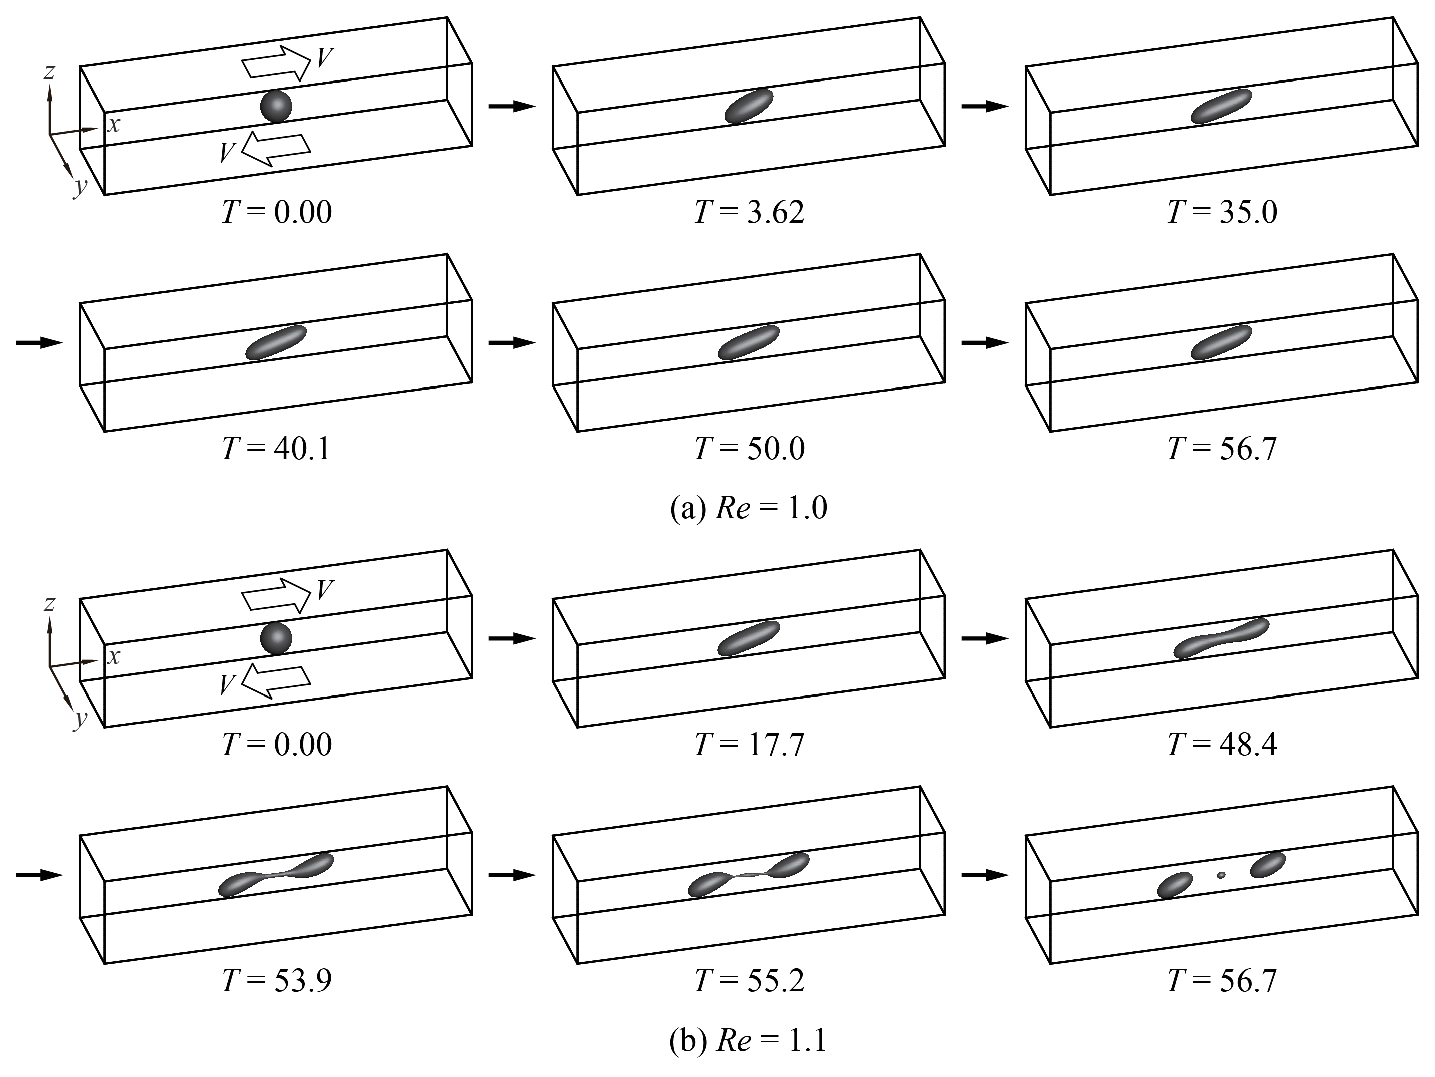
\includegraphics[width=\textwidth]{Figure/4-DropBreakEvol}
  \caption{Time evolution of drop deformation and breakup in shear flow at the
           condition of $Ca=0.3$ with (a) $Re=1.0$ and (b) $Re=1.1$.  The
	   ``drop'' critical Reynolds number corresponding to $Ca=0.3$ is
	   $1.0<Re_{\rm c}<1.1$.
	   ($\lambda$ = $\eta$ = 1.0)}
 }
  \label{fig:DropBreak}
\end{figure}
%\end{comment} 
%
To illustrate the differences in deformation and breakup between a drop and a bubble around critical conditions, we first present numerical results for drop deformation.  The time evolution of drop deformation and breakup in simple linear shear flow for two conditions is shown in Figure \ref{fig:DropBreak}; the first case, shown in Figure ~\ref{fig:DropBreak}(a), uses $Ca=0.3$ and $Re=1.0$, while the second case, depicted in Figure ~\ref{fig:DropBreak}(b), uses $Ca=0.3$ and $Re=1.1$.  Using a domain size of $\lwh{24}{6}{6}$, in the case with $Re=1.0$, the drop gradually deforms and finally attains a stable deformed state. 

\textcolor{red}
{
After $T$ = 35.0, the drop remains a stable deformed state with $D$= 0.549.  Over the same domain, for the case with $Re=1.1$, the ``mother'' drop elongates over time, and the volume at the ends of the deforming drop expands; both ends become bulb-shaped.  As time progresses, particularly over the time interval $48.4 \leq T \leq 55.2$, a thread-bridge forms between the bulbous ends, and the thread-bridge becomes thinner.  Finally, at around the dimensionless time $T\sim 56.7$, the mother drop breaks up, forming two ``daughter'' drops through the pinch-off; one satellite drop is also generated between the pinched-off daughter drops.  
}

\subsection{Bubble deformation and breakup}
%  -----------------------------------------------------------------------------
% 
%\begin{comment} 
\begin{figure}%[h!]
  \centering
  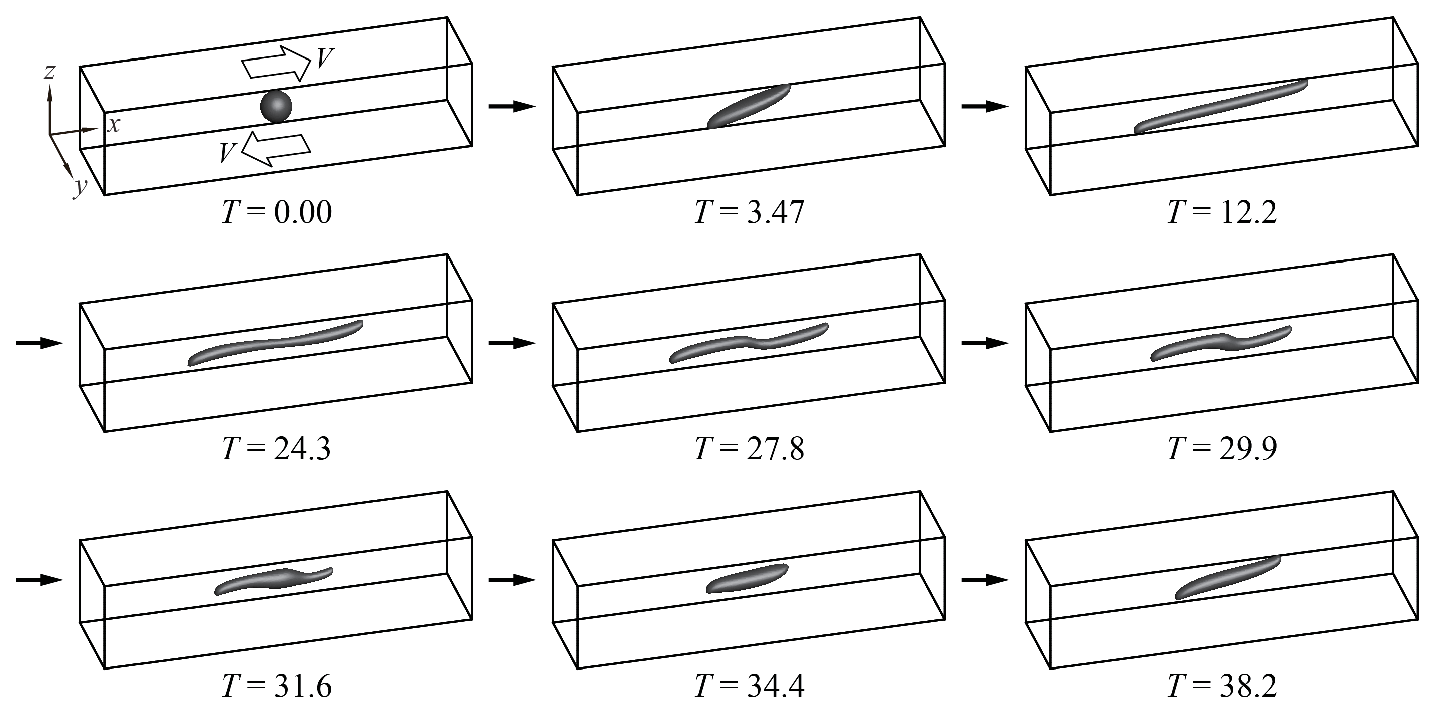
\includegraphics[width=\textwidth]{Figure/5-BubbleBreakCa0p3Re92}
  \caption{Time evolution of bubble deformation in shear flow at the
           condition of $Ca=0.3$ and $Re=92$.  
	   The ``bubble'' 
	   critical Reynolds number corresponding to $Ca=0.3$ is
	   $92<Re_{\rm c}<93$.  In contrast to the drop deformation case,
           when $Re$ is slightly below $Re_{\rm c}$
           (See Figure \ref{fig:DropBreak} $Re=1.0$ for the drop case), 
           the bubble shape will
           not reach a steady shape, instead the bubble shape alternates
           between the shapes ``slightly stretched'' ($T=3.47$),
           fully stretched and ``doglegged'' ($T=27.8$) and ``almost''
           back to the original ``slightly stretched'' case 
           ($T=34.4$). 
           ($\lambda = 1.2 \times 10^{-3}$, $\eta < 1.0 \times 10^{-3}$) 
	   }
  \label{fig:BubbleBreakCa0p3Re92}
\end{figure}
%\end{comment} 
%
%\begin{comment}
\begin{figure}%[h!]
  \centering
  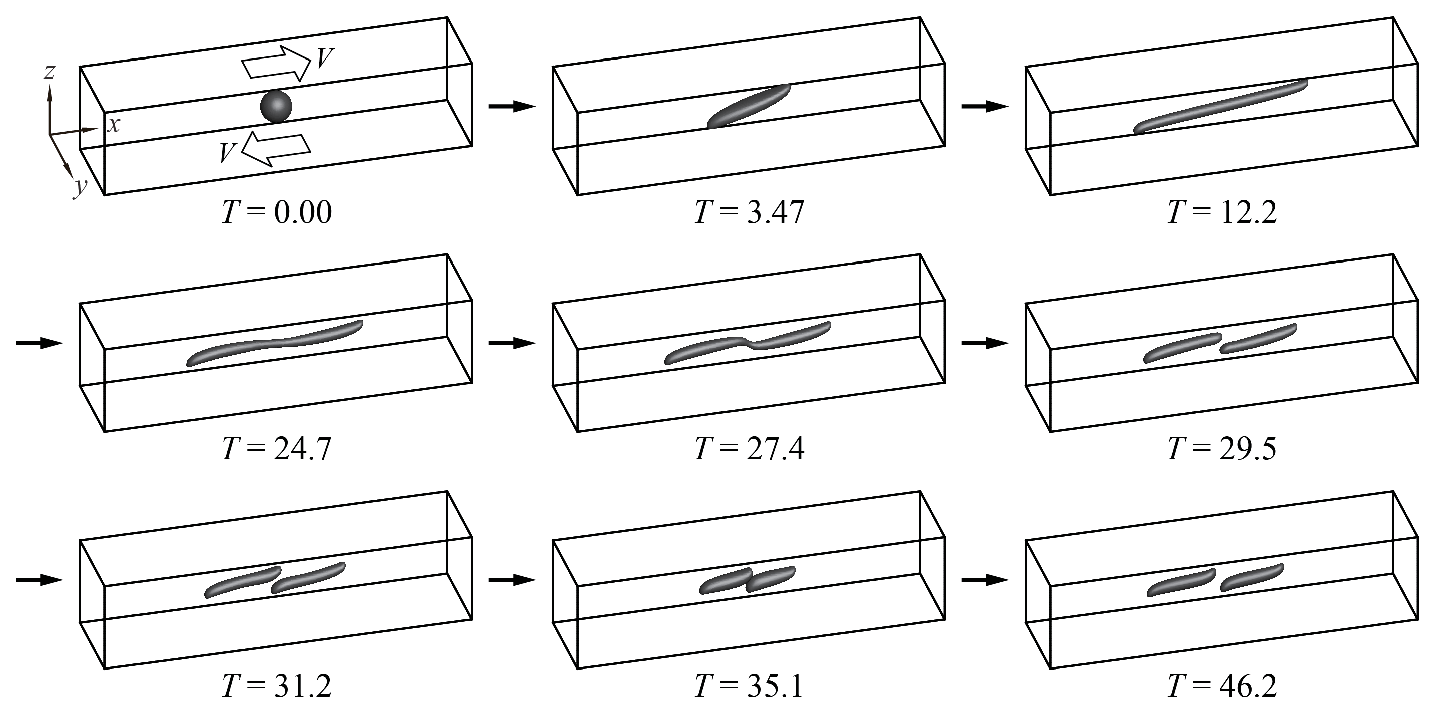
\includegraphics[width=\textwidth]{Figure/6-BubbleBreakCa0p3Re93}
  \caption{Time evolution of bubble deformation in shear flow at the
           condition of $Ca=0.3$ and $Re=93$.
	   The ``bubble'' 
	   critical Reynolds number corresponding to $Ca=0.3$ is
	   $92<Re_{\rm c}<93$.
           ($\lambda = 1.2 \times 10^{-3}$, $\eta < 1.0 \times 10^{-3}$) 
	   }
  \label{fig:BubbleBreakCa0p3Re93}
\end{figure}
%\end{comment} 
%
Next, we present numerical results that illustrate the conditions that lead to bubble deformation without breakup and conditions where the bubble deforms and ultimately breaks up.  The time evolution of shear-induced bubble deformation without breakup at the condition of $Ca=0.3$ and $Re=92$ is depicted in Figure~\ref{fig:BubbleBreakCa0p3Re92} and the bubble breakup process with flow condition of $Ca=0.3$ and $Re=93$ is illustrated in Figure~\ref{fig:BubbleBreakCa0p3Re93}.  The results indicate that the critical Reynolds number is approximately $Re_{\rm c}$ = 93 (with $Ca=0.3$).  A comparison with the drop breakup dynamics presented in Section~\ref{sec:DropBreak} and the corresponding processes for bubble deformation and breakup exhibit very distinct features.  First, we note that a relatively large shear force magnitude is required for bubble breakup ($\lambda = 1.2 \times 10^{-3}$, $\eta < 1.0 \times 10^{-3}$) compared with the case of the drop ($\lambda$ = $\eta$ = 1). Then, for the same value of $Ca=0.3$, the critical Reynolds number for the bubble is around 85 times larger than that for the drop.  Focusing on the bubble dynamics with no-breakup (Figure~\ref{fig:BubbleBreakCa0p3Re92}), the results show that the bubble is noticeably elongated in the $x$-direction at the early stages ($T \leq 24.3$) of bubble deformation, but the bubble does not develop the bulb-like shape (large volume areas) at both ends as observed in the drop deformation process.  It is also evident that the ends of the deforming bubble develop cusped shapes under the influence of the strong shear flow.

\textcolor{red}
{
In providing a more detailed description, very large shear forces are required to deform the bubble because $\lambda \simeq 0$ and $\eta \simeq 0$.  Thus, the bubble undergoing large shear forces at $T > 0$ is largely stretched along the shear flow direction, and the very long elongated bubble with cusped shapes is formed.  Accordingly, the bubble finally breaks up through the elongated shape without forming a bulb-like shape.  A noteworthy feature of the non-breaking bubble is that it does not settle into a deformed stable state as in the case of drop deformation presented in Figure~\ref{fig:DropBreak}(a).  After an initial elongation process, the bubble enters a shrinking phase ($T = 27.8$) where the doglegged shape formed at the center of the bubble returns to a smaller deformed shape ($T = 34.4$) that is similar to its earlier shape ($T=3.47$).  However, when we compare the early deformed bubble shape at $T = 3.47$ with the shape at $T = 34.4$, it is clear that the shapes are not identical.  Following the shrinking phase, the bubble stretches again ($T = 38.2$) and oscillates between its elongated shape and shortened geometry.  
}

%
%\begin{comment} 
\begin{figure}%[h!]
  \centering
  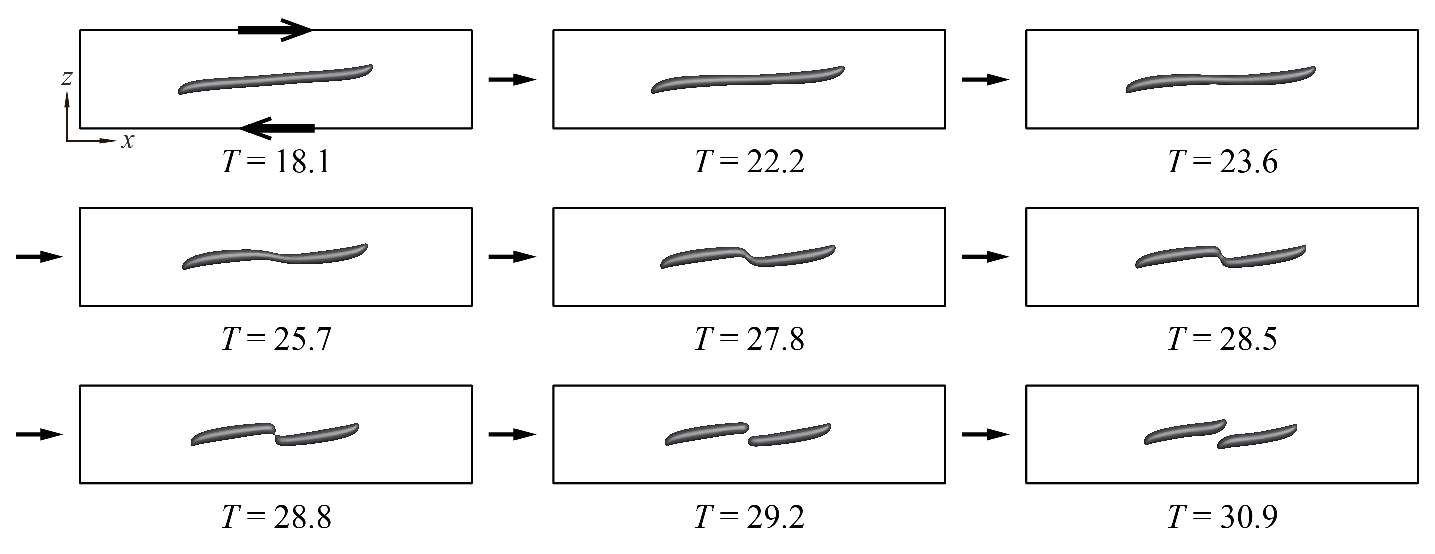
\includegraphics[width=\textwidth]{Figure/7-BubBreakCa0p3Re93Detail}
  \caption{Detail of bubble breakup process in shear flow at the condition
           of $Ca=0.3$ and $Re=93$.
	   The ``bubble'' 
	   critical Reynolds number corresponding to $Ca=0.3$ is
	   $92<Re_{\rm c}<93$.
           ($\lambda = 1.2 \times 10^{-3}$, $\eta < 1.0 \times 10^{-3}$) 
	   }
  \label{fig:BubBreakCa0p3Re93Detail}
\end{figure}
%\end{comment} 
%
\textcolor{red}
{
For the case of bubble breakup (Figure~\ref{fig:BubbleBreakCa0p3Re93}), we observe that the deformation process is almost the same as the no-breakup case until the doglegged shape is formed at $T \sim 27.4$. The bubble finally breaks during the time interval $27.7 \leq T \leq 29.5$.  For a closer examination of the bubble breakup process, a detailed panel of cross-sectional slices in the $xz$-plane through the bubble shape center is presented in Figure~\ref{fig:BubBreakCa0p3Re93Detail}.  The images displayed in Figure~\ref{fig:BubBreakCa0p3Re93Detail}, which are taken at shorter time intervals than those shown in Fig.~\ref{fig:BubbleBreakCa0p3Re93}, reveal that the bubble breaks up into two daughter bubbles due to the pinch off at the thread-bridge part of the doglegged shape during the shrinking process ($T = 28.5 \sim 28.8$).  After breaking up, the two daughter bubbles migrate to the center: the left daughter bubble moves toward the right side of the domain and the right daughter bubble moves to the left side (see results for $T = 29.5 \sim 35.1$ in Figure~\ref{fig:BubbleBreakCa0p3Re93} and for $T = 28.8 \sim 30.9$ in Figure~\ref{fig:BubBreakCa0p3Re93Detail}).  The two daughter bubbles then momentarily congregate near the domain center ($T = 35.1$ in Figure~\ref{fig:BubbleBreakCa0p3Re93}), before they slowly start to separate: the left daughter bubble moves to the left, and the right daughter bubble moves to the right ($T = 46.2$ in Figure~\ref{fig:BubbleBreakCa0p3Re93}).  The results demonstrate that the bubble breakup process is markedly different from the analogous drop breakup process with $\lambda = 1$ and $\eta =1$. Note that the appearance of deformation and breakup of the drop will largely depend on the viscosity ratios.  
}

%% Ohta

\subsection{Shear stress acting on the bubble}
%  -----------------------------------------------------------------------------
%
%\begin{comment} 
\begin{figure}%[h!]
  \centering
% \includegraphics[width=\textwidth]{8-ShearStress}
  \includegraphics[scale=0.4]{Figure/8-ShearStress}
  \caption{Normalized shear stress $\tau^{\ast}$ around a bubble for 
	two Reynolds 
        numbers under the condition of $Ca = 0.3$. The left image shows the 
        shear stress profile at $Re=50$ and the right image at $Re=93$.
   }
  \label{fig:ShearStress}
\end{figure}
%\end{comment} 
%

\textcolor{red}
{
The previous section discussed bubble deformation and breakup. Large deformation and breakup of the bubble are expected to be closely related to the state of shear stress acting on the bubble.  Figure~\ref{fig:ShearStress} shows the shear stress profile around a bubble for two Reynolds numbers under the condition of $Ca = 0.3$: Reynolds number equal to 50 and 93.  The shear stress profile on the left corresponds to the case of $Re = 50$, and the right side shows the shear stress profile for the case of $Re = 93$.  The normalized shear stress, $\tau^{\ast} = \tau / \tau_{0}$, is defined as a ratio of the local shear stress $\tau = \mu_{\rm m}$$\sqrt{2\bmD:\bmD}$ and the apparent shear stress $\tau_{0} = \mu_{\rm m}$$\mathit{\Gamma}$.  In this study, for a given $Ca$ condition, the same value of $\tau_{0}$ is used regardless of $Re$.  For the case of $Re = 50$, the bubble reached a deformed stable state, and the shear stress profile around the bubble was drawn after the bubble attained a stable deformed state.  As observed in previous sections, when the value of $Re$ is slightly below the critical $Re$ condition, the bubble does not settle into a deformed stable state. Instead, it alternates in an elongation and contraction process.  The shear stress profile for the case of $Re$ = 93 was depicted when the bubble sufficiently elongated ($T$ = 14.9).  In comparison to the $Re=50$ case on the left, the right image in Fig.~\ref{fig:ShearStress} ($Re=93$) shows a higher shear stress profile near the bubble endpoints as it undergoes an elongation state in the process toward breakup.  The value of the maximum shear stress for the case of $Re = 50$ is $\tau ^{\ast} \approx 6$ and the maximum shear stress for the case of $Re = 93$ at the moment shown in Fig.~\ref{fig:ShearStress} has the value of $\tau ^{\ast} \approx 8$.  The shear stress profile in Fig.~\ref{fig:ShearStress} (color contour) is drawn in the range from $\tau^{\ast} = 1$ to $\tau ^{\ast} = 8$, but, for emphasis, shear stress regions with $\tau ^{\ast} \geqq 6$ are illustrated in red.  As shown in the figure, the strongest shear stresses are concentrated on the ends of the bubble for both $Re$ conditions.  This indicates that the strong shear stresses acting on the ends of the bubble are responsible for much of the bubble stretching.  It is important to note that the magnitude of the shear stress acting on the ends of the bubble for the case of $Re = 93$ is much larger than that for the case of $Re = 50$.  
}

We also observed that the shear stress inside the bubble was very small relative to that of the matrix fluid due to the bubble's very small density and viscosity. Since the force of strong shear stresses acting on the ends of the bubble is difficult to transfer across the interface, a sufficiently large $Re$ condition is required for large bubble deformations.

\par\noindent

In summary, we discover that for the Reynolds number sufficiently below the critical value, a relatively quick, unsteady elongation period gives way to a steady state (with no break up).  On the other hand, for the Reynolds number close to the critical Reynolds number, there is a prolonged, unsteady elongation period in which periodic motion is observed, and the deformation parameter $D$ is close to one.  The ``vacillating'' behavior cannot last forever; ultimately (perhaps stochastically!), the bubble will either settle down or break.  Regardless of the outcome, this vacillating behavior will always occur near the critical Reynolds number.  In other words, irrespective of the result, we claim, using the grid resolution of $R/16$, that one is assured of being within 3 percent of the critical Reynolds number (see Figure \ref{fig:DeEvolution}).  We hypothesize that there will always be ``vacillating'' behavior if one is sufficiently close to the critical Reynolds number.  In other words, given an almost infinite supply of computational resources, as one hones in closer and closer to the critical Reynolds number, a ``tug of war'' will be observed between the surface tension force trying to pull the bubble together versus the wall driven shear stress trying to pull the bubble apart.

\subsection{Velocity field outside and inside the breaking bubble}
%  -----------------------------------------------------------------------------
%
%\begin{comment} 
\begin{figure}[h!]
  \centering
  \includegraphics[width=\textwidth]{Figure/9-BubbleFieldCa0p3Re93}
  \caption{Fluid velocity field outside and inside the breaking bubble in
           shear flow at the condition $Ca=0.3$ and $Re=93$.
	   The ``bubble'' 
	   critical Reynolds number corresponding to $Ca=0.3$ is
	   $92<Re_{\rm c}<93$.
           ($\lambda = 1.2 \times 10^{-3}$, $\eta < 1.0 \times 10^{-3}$) 
	   }
  \label{fig:BubbleFieldCa0p3Re93}
\end{figure}
%\end{comment} 
%
\textcolor{red}
{
This section considers the fluid flow velocity field outside and inside the bubble during the shear-induced breakup process.  Detailed velocity fields of the deforming and breaking drop have already been presented in a few references (\citet{LiRenRen00, RenCri01-1}).  The behavior of the breakup process will influence the velocity fields for the drop and the bubble, so the velocity fields for the drop and the bubble are not similar.  Figure~\ref{fig:BubbleFieldCa0p3Re93} shows the velocity fields outside and inside the bubble at cross-sectional slices in the $xz$-plane for a flow condition of $Ca = 0.3$ and $Re = 93$.  Regions around the bubble with a higher density of velocity vectors correspond to the level-1 grid portion of the AMR structure.  The simulation results show that the velocity field inside the bubble is notably distinct from the surrounding flow field on the bubble's exterior.  The cross-sections at $T=12.2$ and $T=18.1$, taken during the elongation phase, show how shear forces at the lower and upper halves of the bubble act along the bottom and top surfaces, respectively, to deform the interface.  Near the left and right edges of the bubble, inward interior flows (that point toward the bubble center) begin to develop.  Strong shearing forces in the exterior near the bottom-left-end and top-right-end of the bubble interact with the interior flow field through the boundary to create cusped shapes at the bottom-left and top-right ends of the bubble. At the same time, the interface is laterally elongated in the $x$-direction.  During the shrinking process, which occurs for $23.6 \leq T \leq 27.8$, inward flows within the bubble extend over a wider region and are no longer localized near the bubble edges.  Then, we observe that circulating flows form at the thread-bridge part of the doglegged bubble shape over the time interval $[25.7, 27.8]$.  During the breakup process ($T \sim 28.8$), higher-intensity inward flows are formed inside the bubble, near the pinch-off region, that are naturally larger than the surrounding interior flows and which are inextricably associated with the bubble migration illustrated in Figs.~\ref{fig:BubbleBreakCa0p3Re93} and~\ref{fig:BubBreakCa0p3Re93Detail}.  As time proceeds further ($T =  46.2$), distinct inward flows are formed inside the daughter bubbles; the bubbles then migrate toward the side walls.  For example, considering the left daughter bubble, we see that the mechanism responsible for this movement results from larger shear forces acting on the bottom-left end than those in the top-left end.
}

\subsection{Effect of surface tension on bubble deformation and breakup}
%  -----------------------------------------------------------------------------
%
%\begin{comment} 
\begin{figure}%[h!]
  \centering
  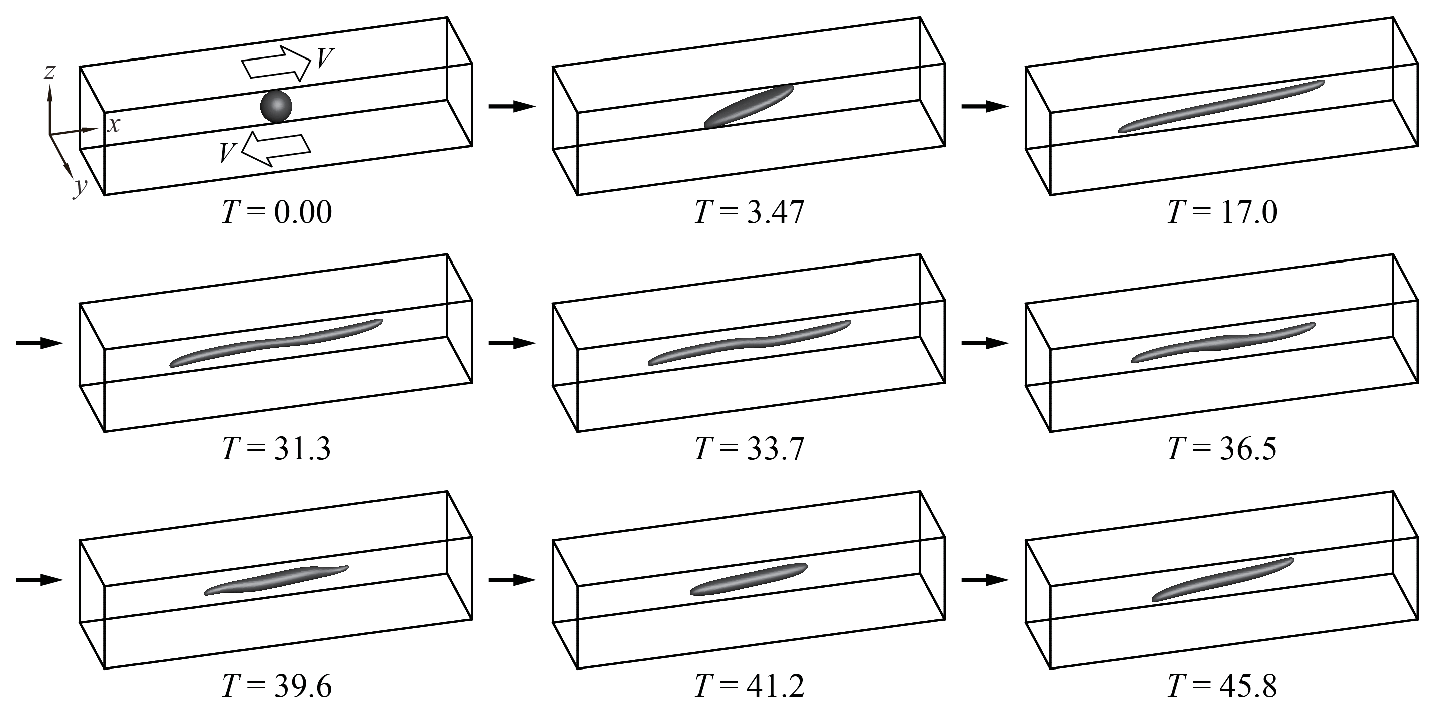
\includegraphics[width=\textwidth]{Figure/10-BubbleDeformCa0p8Re42}
  \caption{Time evolution of bubble deformation in shear flow at the 
           condition of $Ca=0.8$ and $Re=42$.
	   The ``bubble'' 
	   critical Reynolds number corresponding to $Ca=0.8$ is
	   $42<Re_{\rm c}<43$.
           ($\lambda = 1.2 \times 10^{-3}$, $\eta < 1.0 \times 10^{-3}$) 
	   }
  \label{fig:BubDefCa0p8Re42}
\end{figure}
%\end{comment} 
%
%\begin{comment} 
\begin{figure}%[h!]
  \centering
  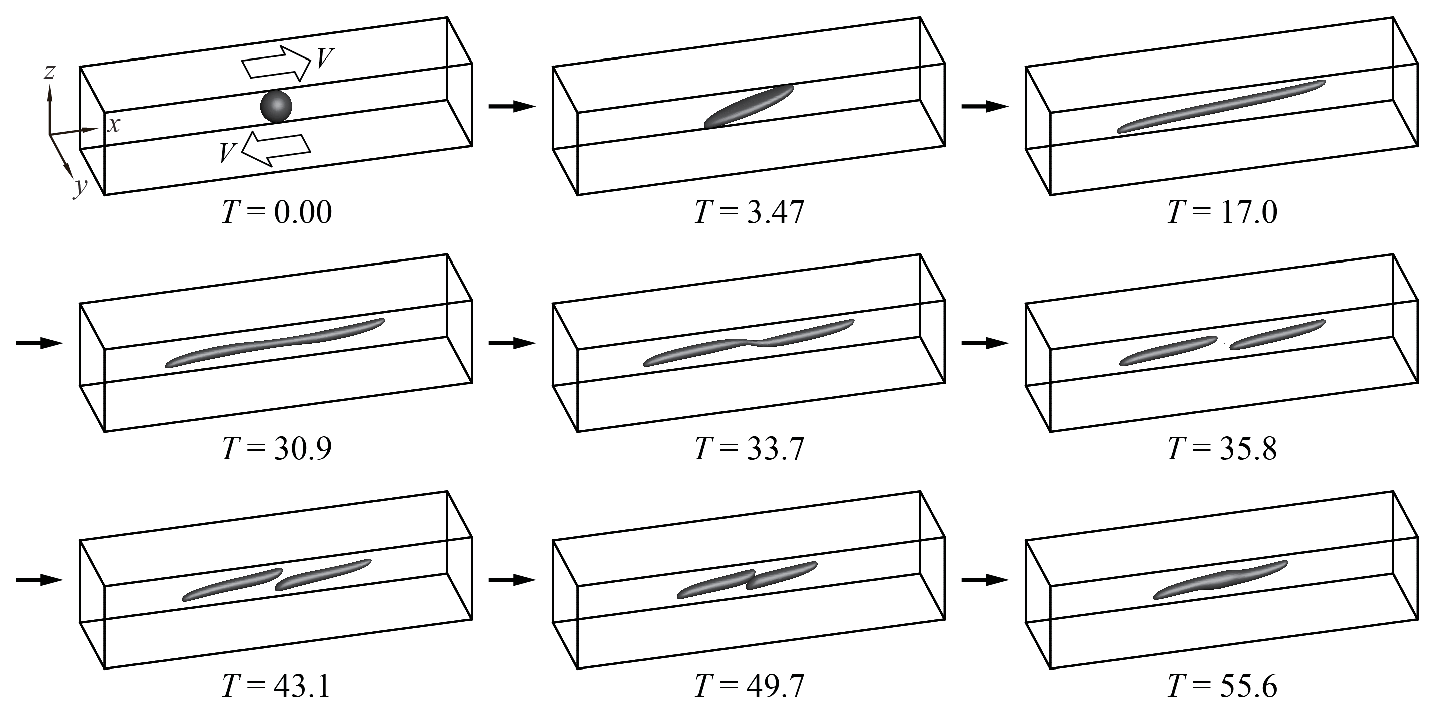
\includegraphics[width=\textwidth]{Figure/11-BubbleBreakCa0p8Re43}
  \caption{Time evolution of bubble deformation in shear flow at the 
           condition of $Ca=0.8$ and $Re=43$.
	   The ``bubble'' 
	   critical Reynolds number corresponding to $Ca=0.8$ is
	   $42<Re_{\rm c}<43$.
           ($\lambda = 1.2 \times 10^{-3}$, $\eta < 1.0 \times 10^{-3}$) 
	   }
  \label{fig:BubBrkCa0p8Re43}
\end{figure}
%\end{comment} 
%
%It means that the effect of the surface tension for the condition of $Ca = 0.8$
%is smaller than that for the condition of $Ca = 0.3$.
%
In previous sections, we considered numerical simulations of bubble deformation and breakup with a capillary number $Ca = 0.3$.  In this section, we examine the case of $Ca=0.8$.    We investigate the effect of interfacial tension on bubble deformation and breakup.  Using $Ca=0.8$ for both cases, Figures~\ref{fig:BubDefCa0p8Re42} and~\ref{fig:BubBrkCa0p8Re43} present the time evolution of shear-induced bubble deformation and breakup with $Re=42$ and $Re=43$, respectively.  We note that the bubble critical Reynolds number is around $Re_{\rm c} \approx 43$, whereas $Re_{\rm c} \approx 0$ for the corresponding case of the drop with $\lambda$ = $\eta$ = 1 (see e.g.~\citet{LiRenRen00}).  Note that $Re_{\rm c}$ for $Ca = 0.8$ is smaller than that for the condition of $Ca = 0.3$ since the bubble at $Ca = 0.8$ is more elastic due to the weaker effect of surface tension in this case.  The results shown in Figs.~\ref{fig:BubDefCa0p8Re42} and~\ref{fig:BubBrkCa0p8Re43} indicate that the bubble deformation and breakup process for the condition of $Ca = 0.8$ is analogous to that for $Ca = 0.3$.  For the case of bubble deformation without breakup (Fig.~\ref{fig:BubDefCa0p8Re42}), the bubble initially assumes a long elongated shape along the $x$-direction at around $T=17.0$. The bubble then enters a compression stage over the time interval $[31.3,41.2]$ and then elongates again at $T = 45.8$.  On the other hand, for the case of bubble breakup (Fig.~\ref{fig:BubBrkCa0p8Re43}), an initial elongation phase is followed by a doglegged shape formation at $T=33.7$.  After that, the bubble ruptures from the thread-bridge part of the doglegged shape, producing two daughter bubbles ($T = 35.8$).  The two daughter bubbles formed after the breakup move to the central area ($T = 49.7$) as in the case of $Ca = 0.8$ and $Re = 93$. Still, the two bubbles eventually coalesce in a region approximately centered in the computational domain ($T = 55.6$).  We note that bubbles may coalesce after breaking up in a real experimental setting due to slight deviations in flow conditions and states.  Although the process of bubble deformation and breakup for flow conditions with $Ca = 0.3$ and $Ca = 0.8$ are similar, a pronounced difference is that the bubble for $Ca = 0.8$ is more elongated and slender than that for $Ca = 0.3$ due to the smaller effect of surface tension for $Ca = 0.8$.


Table~\ref{tab:CaRecComparison} lists, for representative $Ca$ values, the corresponding critical Reynolds number, $Re_{\rm c}$, for shear-induced bubble breakup.  The data in Table~\ref{tab:CaRecComparison} corresponds to $\lambda = 1.2 \times 10^{-3}$, $\eta < 1.0 \times 10^{-3}$, $0.3<Ca<1$, and the initial/boundary conditions are given by (\ref{IC_BC}).  The results in Table~\ref{tab:CaRecComparison} indicate that sufficiently large shear forces are required for bubble breakup, even for large capillary numbers.  In Figure~\ref{fig:CaRecFit} we plot the smooth interpolant of the data given in Table~\ref{tab:CaRecComparison} and make the hypothesis that given a new data point, $(Ca,Re)$, shear-induced bubble break up will occur if the point $(Ca,Re)$ is above the given critical curve, and the bubble will not break if the $(Ca,Re)$ pair is below the critical curve.  For comparison, a critical curve for the drop with $\lambda =\eta = 1$ is also indicated in Fig.~\ref{fig:CaRecFit}.  Including breakup and no-breakup critical curves for both the drop and the bubble will facilitate future identification of $Re_{\rm c}$ numbers and, thus, a complete general critical curve for a wide range of $Ca$ numbers.

%{\color{red} it seems like the above passage is still a work in progress?}
%Yes. I have been suspending computations for bubbles because I have been
%focussing on non-Newtonian cases, but I have a plan for restarting again.

\begin{table}[tbh]
\caption{Shear-induced bubble breakup for various flow 
	conditions described in terms
        of column pairs of critical Reynolds numbers and 
	corresponding capillary numbers.
        ($\lambda = 1.2 \times 10^{-3}$, $\eta < 1.0 \times 10^{-3}$) 
	}
\label{tab:CaRecComparison}
\footnotesize
\center
\begin{tabular}{ c  c  c  c  c }
\hline
\hline
Capillary number $Ca$            & 0.3  & 0.5  & 0.8  & 1.0  \\
Critical Reynolds number $Re_{\rm c}$  & 93   & 67   & 43   & 35   \\
\hline
\hline
\end{tabular}
\end{table}

%% variance for X^T X c = b
%% (S/(n-m)) (X^T X)^{-1}
%\begin{comment} 
\begin{figure}%[h!]
  \centering
% \includegraphics[width=\textwidth]{12-CaRecFit}
  \includegraphics[scale=0.6]{Figure/12-CaRecFit}
  \caption{A plot of the critical Reynolds number versus capillary number
	for the data listed in Table~\ref{tab:CaRecComparison}.  
	$\lambda = 1.2 \times 10^{-3}$, 
	$\eta < 1.0 \times 10^{-3}$, $0.3<Ca<1$, and
        the initial/boundary conditions are given by (\ref{IC_BC}).
	Given a new data point, $(Ca,Re)$, one
	can reliably predict whether the 
	given $(Ca,Re)$ pair will result in shear
	induced bubble break-up or not.  Note, for the ``Drop delineation
	curve,'' $\lambda=\eta=1$.
	   }
  \label{fig:CaRecFit}
\end{figure}
%\end{comment} 
%

%  -----------------------------------------------------------------------------
\section{Conclusions}
%  -----------------------------------------------------------------------------
\textcolor{red}{
The bubble deformation and breakup process in liquid due to a driving simple linear shear flow was explored numerically using the CLSVOF computational method.  In this study, the critical Reynolds number $Re_{\rm c}$, at which bubble breakup first occurs, was determined for several flow conditions, and the differences between the morphology of bubble deformation and breakup were compared with the analogous morphology of drop deformation and breakup.
}

\textcolor{red}{
The numerical results revealed significant differences between bubble deformation and breakup and the corresponding drop dynamics.  For the case of a bubble, it was discovered that much stronger shear flows are necessary to induce interface breakup compared with a drop immersed in a similar flow field.  That is, a much larger Reynolds number flow is required to induce bubble breakup.  The steps leading to bubble breakup were similar throughout the $Ca$ number range considered in our computations: the bubble underwent a similar breakup mechanism in which rupture occurred at a thread-bridge part that followed a doglegged shape formation stage.  For bubble deformation without breakup, near $Re_{\rm c}$, the bubble did not maintain a stable deformed shape, unlike drop deformation near the critical Reynolds number.  The bubble exhibited pronounced underdamped behavior: the bubble oscillated between elongating and shrinking motions for non-rupturing flow conditions.  At the same time, bubble deformation under smaller $Re$ conditions ($< Re_{\rm c}$) led to a stable state.  Compared with the drop, we attribute the significant differences in morphology for the bubble undergoing breakup to the density and viscosity ratio.  Due to the bubble's very small density and viscosity, it is comparatively difficult to transfer the shear stresses acting on the ends of the bubble across the interface.
}

\textcolor{red}{
There are several directions for future work.  In the present work, we varied the capillary number and Reynolds number to study bubble deformation and breakup morphology in the presence of a simple shear flow.  For the future, one can also vary (i) the viscosity ratio, (ii) the effect of the initial shape of the bubble\cite{ohta2005computational}, (iii) the magnitude and direction of the gravitational force, (iv) the non-Newtonian properties of the ``matrix'' liquid, (v) bubble deformation and breakup due to a shear flow in a T junction\cite{FRENSE2024120579}, (vi) bubble deformation and breakup confined shear flow (see \cite{gupta2014deformation} for the drop case), and (vii) bubble deformation and breakup due to non-uniform shear flow (see \cite{chin1980studies} for the drop case).
}


%\bibliography{apssamp}% Produces the bibliography via BibTeX.
\bibliographystyle{elsarticle-harv} 
\bibliography{Bubble-deformation}

%  -----------------------------------------------------------------------------
%  -----------------------------------------------------------------------------
\end{document}
%
% ****** End of file apssamp.tex ******
